\documentclass[lettersize,journal]{IEEEtran}
\usepackage{amsmath,amsfonts}
\usepackage{amssymb}
\usepackage{algorithmic}
\usepackage{array}
\usepackage[caption=false,font=footnotesize,labelfont=sf,textfont=sf]{subfig}
\usepackage{textcomp}
\usepackage{sidecap}
\usepackage{stfloats}
\usepackage{url}
\usepackage{verbatim}
\usepackage{graphicx}
\hyphenation{op-tical net-works semi-conduc-tor IEEE-Xplore}
\def\BibTeX{{\rm B\kern-.05em{\sc i\kern-.025em b}\kern-.08em
    T\kern-.1667em\lower.7ex\hbox{E}\kern-.125emX}}
\usepackage{balance}
\usepackage{xcolor}
\usepackage{caption}
\usepackage{bm}
\usepackage{booktabs}
% \usepackage[caption=false, font=footnotesize]{subfig}

% to fix undefined citations
% \usepackage[backend=biber,style=ieee]{biblatex}

% \addbibresource{references.bib}

\newcommand{\ihat}{\hat{\imath}}
\newcommand{\jhat}{\hat{\jmath}}
\newcommand{\khat}{\hat{k}}
\newcommand{\q}{\bm q}
\newcommand{\qd}{\dot{\bm q}}
\newcommand{\qdd}{\ddot{\bm q}}
\newcommand{\qnd}{\dot{q}}
\newcommand{\qndd}{\ddot{q}}
\newcommand{\x}{\bm x}
\newcommand{\xd}{\dot{\bm x}}
\newcommand{\xdd}{\ddot{\bm x}}
\newcommand{\xddd}{\dddot{\bm x}}
\newcommand{\xds}{\dot{x}}
\newcommand{\xdds}{\ddot{x}}
\newcommand{\y}{\bm y}
\newcommand{\yd}{\dot{\bm y}}
\newcommand{\ydd}{\ddot{\bm y}}
\newcommand{\yddd}{\dddot{\bm y}}
\newcommand{\yds}{\dot{y}}
\newcommand{\ydds}{\ddot{y}}
\newcommand{\eb}{\bm e}
\newcommand{\ebd}{\dot{\bm e}}
\newcommand{\ebdd}{\ddot{\bm e}}
\newcommand{\omegab}{\bm \omega}
\newcommand{\omegabd}{\dot{\bm \omega}}
\newcommand{\omegabdd}{\ddot{\bm \omega}}
\newcommand{\vb}{\bm v}
\newcommand{\vbd}{\dot{\bm v}}
\newcommand{\rb}{\bm r}
\newcommand{\rbd}{\dot{\bm r}}
\newcommand{\s}{\bm s}
\newcommand{\sd}{\dot{\bm s}}
\newcommand{\taub}{\bm \tau}


%%%%%%

\begin{document}

%\title{Anticipatory Intent Detection for Adaptive Trajectory Generation in Perturbed Robot-to-Human Handovers}
\title{Should I Stay or Should I Go: Anticipatory Intent Prediction for Adaptive Robot-to-Human Handover}
%\title{Should I Stay or Should I Go: Anticipatory Intent Prediction for Adaptive Robot-to-Human Handover in (Perturbed) Dynamic Scenarios}
%\title{Should I Stay or Should I Go: Anticipatory Intent Prediction for Perturbed Robot-to-Human Handover}

\author{Francesco Iori, Gojko Perovic, Matteo Conti, Marco Controzzi, Egidio Falotico
\thanks{This work is supported by the European Commission under the Horizon2020 framework program for Research and Innovation under the APRIL (870142) and HBP (SGA3 945539) projects.}}


\markboth{Journal of \LaTeX\ Class Files,~Vol.~18, No.~9, September~2020}%
{How to Use the IEEEtran \LaTeX \ Templates}

\maketitle

\begin{abstract}
The handover of objects is a fundamental cooperative action in Human-Robot Collaboration (HRC) tasks, requiring the interplay of multiple skills such as perception, coordination, and adaptation.
We present Anticipatory Intent Prediction (AntIP), a novel method for generating adaptive robot handover trajectories that account for unmodeled perturbations during the handover.
AntIP draws inspiration from biological anticipatory control to detect human engagement during the handover, dynamically adjusting the trajectory to slow down or stop when perturbations are detected and resuming once the interaction continues. The method requires minimal perception data, making it computationally efficient, practical to deploy, and adaptable for various handover scenarios. Experimental evaluations demonstrate the system's robustness in handling both standard and perturbed handover conditions,  offering a solution for safer and fluent human-robot interaction.
The videos of the controller in the perturbed interaction scenario are available at \url{https://fraiori0.github.io/antip-handover/}
\end{abstract}

\begin{IEEEkeywords}
Human-Robot Collaboration, Object Handover, Anticipatory Control, Trajectory Generation, Dynamical System.
\end{IEEEkeywords}

\section{Introduction}
\label{sec:introduction}

\noindent \IEEEPARstart{T}HE handover of objects represents a fundamental cooperative action and an essential component of many foreseeable Human-Robot Collaboration (HRC) tasks.
While trivial for humans, the handover of an object requires the interplay of multiple different skills, such as perception, coordination, anticipation, adaptation, grasping, and more \cite{ortenzi_object_2021}.
% Due to its relevance, multiple implementations of methods for robot-human handover have been proposed, each focusing on a subset of the multiple capabilities that are required \cite{ortenzi_object_2021}.
Due to the interactive nature of the action, when performing handovers humans anticipate the movement of their partner and can adjust accordingly \cite{controzzi_humans_2018, huber_spatiotemporal_2013}.
Studies have hinted at humans preferring robotic partners that can replicate such adaptive or anticipatory behavior \cite{huang_adaptive_2015, controzzi_humans_2018, cakmak_human_2011}.
However, controller design can become significantly more complex if the interaction includes disturbances or interruptions.

In this work, we focus on the problem of generating a handover trajectory for the robot (i.e. a trajectory for the reaching movement to deliver/get the object) while considering the presence of perturbations in the execution of the handover itself, a practical scenario that has rarely been considered by the current state of the art \cite{huang_adaptive_2015}.
Here, we refer to a perturbed handover as a handover where an unspecified perturbation occurs, such that the robot should stop the handover or take corrective actions to avoid endangering the human partner while ensuring the fluency of the interaction. 
As a simple example, we can consider the case of a practical joke between two persons: while both start reaching for the handover, one of them stops mid-way (and possibly takes the hand away), making the partner "miss".
While seemingly unrelated, this case exemplifies the problems considered in this work.
First, the "missing" agent should stop reaching for the hand that their partner took back.
Second, if the partner engages back in the handover, the action can typically resume without much effort, with no major disruption or explicit communication.
This work presents AntIP (ANTicipatory Intent Prediction for adaptive handovers) a method to endow a robot with such capabilities, i.e. stopping in case of major perturbations, slowing down in case of minor perturbations, and being able to resume the action should the handover continue, and smoothly modulating a trajectory between handover execution and full-stoppage.
% We note that this setting deviates from what is usually meant by "adaptation" in handover scenarios. In fact, most implementations at the state of the art typically consider adaptation as a way of generating trajectories that are more convenient (e.g. ergonomic) for the human agent \cite{ortenzi_object_2021}.

AntIP addresses adaptation from a low-level control perspective and is inspired by the biological concept of anticipatory control.
According to it, an agent acts according to some expectation (such as a prediction or previous knowledge), and corrective actions are taken only when the execution deviates from what is expected \cite{hoffmann_anticipatory_2004}.
%Inspired by the biological concept of anticipatory control, where corrective actions are taken only when the execution deviates from an expectation,\cite{hoffmann_anticipatory_2004} the proposed approach aims at addressing adaptation from a low-level control perspective.
%In this study we refer to the case of a robotic giver and a human receiver; however, the approach can be readily extended to human-to-robot handovers, as discussed in Sec. \ref{sec:conclusions}.

The contribution of this work is an adaptive trajectory generation method for robot-to-human handovers, able to adapt the robot's speed against potential perturbations while operating normally when no perturbation is present.
AntIP continuously modulates the trajectory between full stoppage and full handover execution and can be tuned to obtain different robot behaviors depending on the intended application, exploiting prediction models that do not require any data from perturbed interactions.
Furthermore, the system operates with minimal perception requirements and is developed to be compatible with common vision pipelines (requiring only the hand position at 30Hz to operate).
%As discussed in later sections, we see the anticipatory-like detection of engagement as an important novelty compared to the state-of-the-art, providing a simple yet robust mechanism for engagement detection.
%Thanks to its peculiarity, the approach removes the requirement for data from perturbed interactions, at the same time making the approach adaptable to suit other trajectory generation schemes or desired reactions (e.g., making the robot go back when disengagement is detected).
%Thanks to this property, anticipatory-inspired modulation is here implemented on a trajectory generation method that can consider directly the other's agent hand as the target, an approach that has already been demonstrated as both practical and robust against the relative configurations of the two agents (e.g., the human does not have to be standing at some specific distance or pose in front of the robot) \cite{prada_implementation_2014, medina_human-inspired_2016}.
%Finally, as the system operates directly at the level of trajectory generation, it can be incorporated into higher-level components that may decide when to start or conclude the whole handover interaction, possibly reducing their requirements.
We perform experimental evaluations to demonstrate the system's robustness in generating and adapting handover trajectories in both standard and perturbed handover conditions.
To the best of the authors' knowledge, this is the first time that a method aimed at unpredictable perturbed conditions in handover scenarios has been demonstrated.

\begin{figure}[t!]
\centering
    \subfloat[\label{fig:frames:1}]{%
        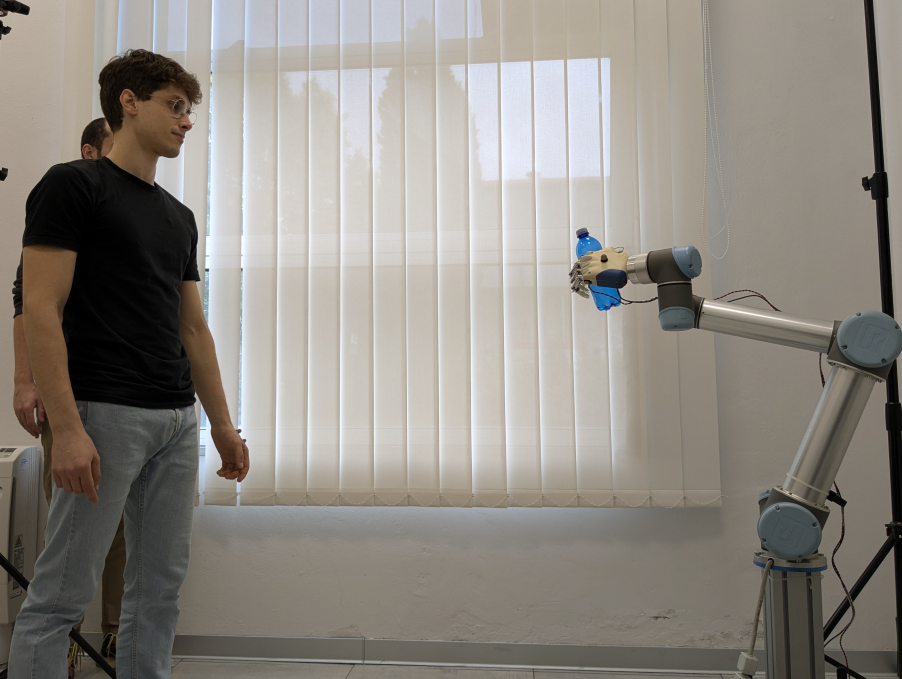
\includegraphics[width=0.49\linewidth]{figs/frames/sample_0_reduced.png}}
    \hfill
    \subfloat[\label{fig:frames:2}]{%
        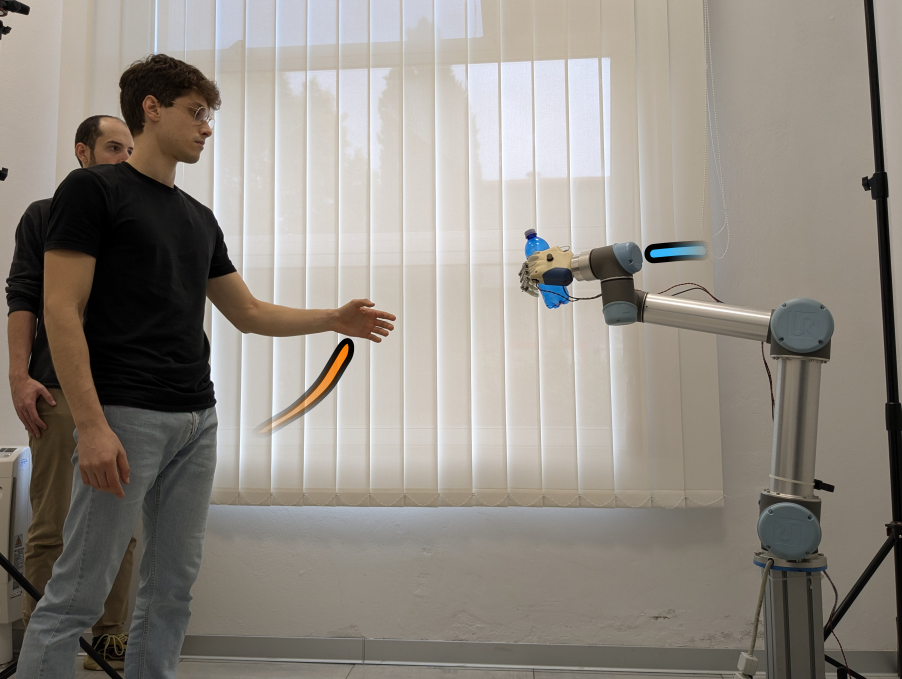
\includegraphics[width=0.49\linewidth]{figs/frames/sample_1_reduced.png}}
    \\
    \subfloat[\label{fig:frames:3}]{%
        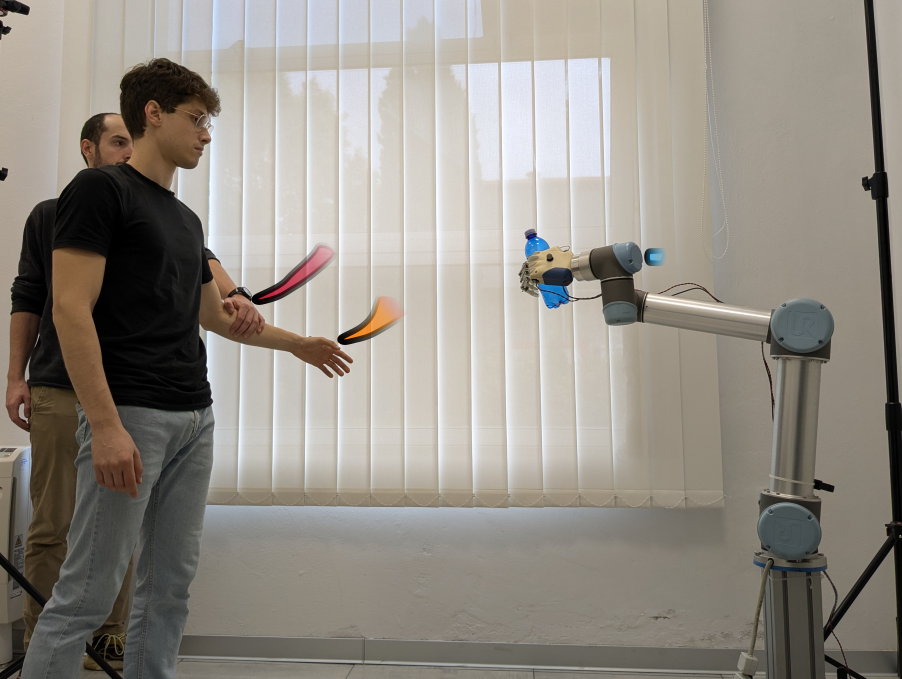
\includegraphics[width=0.49\linewidth]{figs/frames/sample_2_reduced.png}}
    \hfill
    \subfloat[\label{fig:frames:4}]{%
        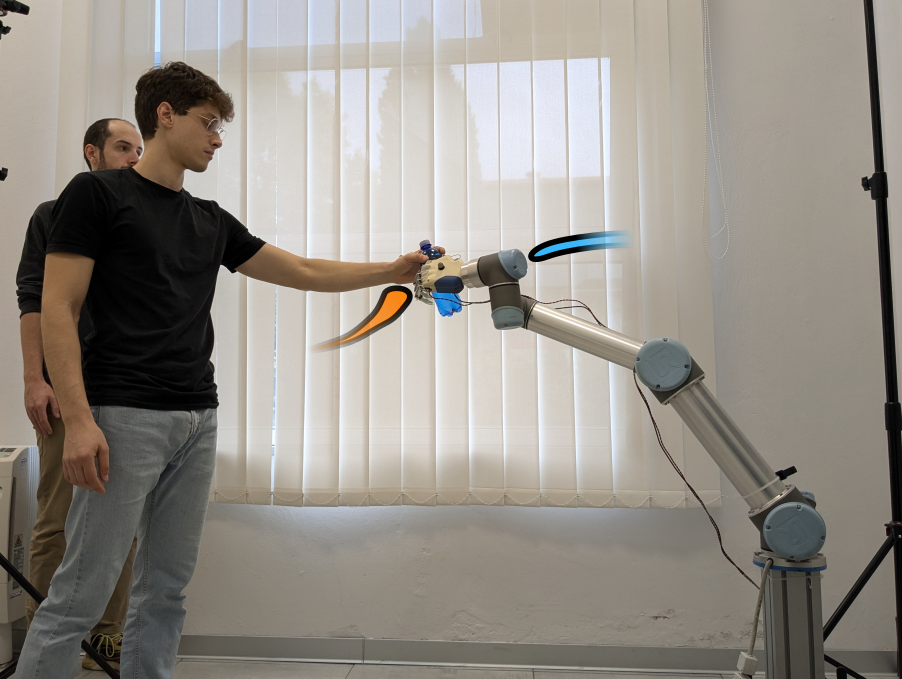
\includegraphics[width=0.49\linewidth]{figs/frames/sample_3_reduced.png}}

    \caption{Frames showing an example of a perturbed scenario, in which the subject's arm is pulled during the handover. 
    The colored traces highlight the relative motion of the hand and the robot between frames.
    The robot is actively executing the handover, with the proposed controller, at all time during the interaction.
    When the perturbation is detected the robot trajectory is slowed down, speeding up again once the participant reaches back for the object.}
    \label{fig:frames:all}
\end{figure}

\section{Related work}

\noindent
%As mentioned before, with the growing interest in developing HRC applications, robotic handover has garnered relative popularity in robotic literature.
%However, seamless human-like handovers still represent a considerable challenge \cite{ortenzi_object_2021}.
We present an overview of the work most related to the proposed approach.
For a broader perspective on the multiple challenges concerning robotic handovers, Ortenzi et al. \cite{ortenzi_object_2021} provide an in-depth treatment focused on robotic applications.

\subsection{Intent in handovers}

\noindent
Handover, by its very nature, involves cooperation between a giver and a receiver, both temporal and spatial, which can be mediated by different (active or passive) forms of explicit and implicit intention cues, both before and during the action \cite{ortenzi_object_2021}.
To this end, robotics applications that make use of various explicit modalities to communicate intent have been proposed: speech \cite{foster_human-robot_2006}, gaze \cite{foster_human-robot_2006}\cite{moon_meet_2014}, tactile feedback \cite{cini_relevance_2021}, and gestures \cite{cakmak_using_2011}.
Implicit forms of communication also play an important role as a means of both predicting the action of the other partner and adjusting one's own behavior according to such prediction (such as for grip force \cite{controzzi_humans_2018} or intention to handover \cite{huber_spatiotemporal_2013} \cite{pan_automated_2017}).
Humans can also directly adjust their trajectories to project intent while performing joint actions \cite{pezzulo_human_2013}, altering the trajectory with respect to assumed default behavior.
Moreover, anticipation can also play a role in the fluency of robot-human handovers \cite{cakmak_using_2011}.

Finally, regarding the perception of cooperation, it has been highlighted how, in human-robot handovers, temporal precision takes priority over spatial one when it comes to user satisfaction \cite{koene_relative_2014}.

As we target a fast-reacting and comparatively simpler system, AntIP exploits only the hand motion of the two agents during the handover.
Previous experiments warrant this choice \cite{iori_dmp-based_2023} \cite{perovic_adaptive_2023} where the hand motion was used to adapt the robot's speed in more restrictive settings (i.e. with a pre-known exchange location), suggesting it can be an informative feature for adaptation.

\subsection{Trajectory Generation for Handover}
\label{subsec:rw:trajectory}

\noindent
Handover trajectories bring a robot's end-effector to the human hand, reaching the final exchange location, or goal, of the handover.
First, we note that a requirement for temporal coordination imposes a requirement for some form of online generation/adaptation of the trajectory, especially in unstructured handover scenarios where perturbations might arise.

A first class of methods for the generation of trajectories for robot-human handover is represented by virtual dynamical systems, applied to generate online a trajectory.
Applications range from relatively straightforward implementations, such as exploiting Dynamical Movement Primitives (DMP) to generate a trajectory that converges to the hand, as a moving target \cite{prada_implementation_2014}; to more complex implementations generating a trajectory to reach a predicted "collision" point \cite{medina_human-inspired_2016}.
This class of methods has also been proven effective in dealing with non-standard scenarios where the agents are not simply placed in front of each other, such as a mechanic reaching from under a car \cite{prada_implementation_2014}.

Another broad class of methods can be found in probabilistic kinematics algorithms, which condition the kinematics of the robot on the present, past, or predicted trajectory of the human and of the robot itself.
In this context, the motion of the human can be interpreted as a form of implicit communication that conditions the robot on how the handover should be executed.
Multiple frameworks are available for this problem, such as Probabilistic Motion Primitives (ProMP) \cite{paraschos_probabilistic_2013}, Interaction Primitives \cite{ben_amor_interaction_2014}, or Interaction Meshes \cite{ho_spatial_2010}, all of which have been applied to the generation of trajectories for HRC tasks, including handover \cite{maeda_probabilistic_2017}, \cite{ben_amor_interaction_2014}, \cite{vogt_system_2017}.
While this kind of approach is capable of producing expressive robot behaviors \cite{maeda_probabilistic_2017}, \cite{ben_amor_interaction_2014}, they often come at the cost of more elaborate perception (to track, and predict the motion of, multiple body segments \cite{ben_amor_interaction_2014}), with an associated cost in the relative size of a training set sufficient to generalize over various handover configurations, scenarios, and conditions.

Other methods have also been presented in the broader context of human-robot interaction, like minimum-jerk motion \cite{huber_human-robot_2008} or planning as optimization of legibility and predictability scores \cite{dragan_effects_2015}; as mentioned above, however, offline planning may significantly interfere with online adaptation during the task.
To alleviate this issue, hybrid methods considering both a global and local planner have also been devised \cite{marturi_dynamic_2019}.

Given 1) the demonstrated practicality of tracking the human hand \cite{prada_implementation_2014} (or a prediction of it \cite{medina_human-inspired_2016}), 2) its straightforward applicability to a wide range of scenarios \cite{prada_implementation_2014}, and 3) its appealing simplicity, AntIP considers an approach based on virtual dynamical systems.
However, the anticipatory intent detection mechanism is of general applicability to modulation of other trajectory generation methods.

\subsection{Reaction to Perturbations}
\label{subsec:rw:reaction}

\noindent
Robotic handover literature seldom considers explicitly situations where the handover could somehow be interrupted or disrupted.
Notably, Huang et al. \cite{huang_adaptive_2015} presented an adaptive controller for a robotic giver that accounts for the human receiver’s occupancy, investigating how it may affect subjective and task performance metrics during a handover.
Unlike AntIP, it is based on a Finite State Machine (FSM), particularly suited to the considered application, which consists of multiple tasks required from the robot (reach, grasp, retrieve, give, handover, retract) in the examined setting of unloading dishes \cite{huang_adaptive_2015}.
In a similar spirit, AntIP exploits a controller that is able to detect perturbations.
However, AntIP focuses on reacting to perturbations while under the assumption of "permanence" of the intention of handover on the robot’s side, i.e., the robot adapts its trajectory while in the "handover" state.
Thus, the interaction is modulated continuously, at the level of trajectory generation instead of on a higher, symbolic, level.
%The practicality of the low-level approach can be considered if we envision that a high-level controller (such as in \cite{huang_adaptive_2015}) could be too slow or fail at recognizing when a handover should be interrupted or adjusted, or in the case of initiating the handover too soon (when the human is potentially distracted).
Importantly, thanks to the anticipatory approach AntIP is able to do so without requiring data from perturbed interactions, i.e., requiring only positive examples.

%On a different note, even if they have not been proposed explicitly for such application, it is worth considering the potential application of probabilistic frameworks to react to perturbations, such as those discussed in subsection \ref{subsec:rw:trajectory}.
%If applied directly to generate the robot motion, they would learn a probability distribution of robot motion conditioned by the observed human motion.
%Such requirements could prove challenging to meet, the issue being the unpredictability and variability of perturbations causing a fast growth of possible scenarios, rapidly increasing the requirements for data and generalization of a model.
%As an example, consider a human reaching for an object and receiving an unexpected push against their arm; the variations in the motion of the two agents would require multiple training examples for one specific perturbation.


%Instead of relying on learned correlations, a controller could detect whether or not the human is engaging in a handover and implement a learned or hard-coded adaptation strategy when it detects that the human is not moving for the handover.
%This conceptual approach is followed here and is akin to the work performed by Huang et al. \cite{huang_adaptive_2015}, where the robot must decide when and how to engage in the handover.

%Such considerations also further contributed to the choice of exploiting only the hand position of the two agents for intent detection, trading off refined behaviors in favor of generalization to multiple scenarios, practicality of the approach, and a lower requirement for data.
%Thanks to the anticipatory-like approach, the method benefits from the specialization of a model on non-perturbed handovers (i.e., a model not predicting correctly in perturbed scenarios), further lowering the requirements on the generalization capabilities of a trained model.

\subsection{Handover-oriented Motion Prediction}
\noindent
The general problem of prediction of human motion has been widely investigated in the literature.
Here we limit our scope to the context of handover applications.

Sidiropoulos et al. \cite{sidiropoulos_human-robot_2021} proposed a DMP-based approach, coupled with an Extended Kalman Filter, to represent possible human trajectories during human-to-robot handovers.
%The predictor consists of a DMP coupled with an Extended Kalman Filter, which estimates the DMP parameters online.
The model is robust to modeling errors in goal estimation; however, these errors can result in incorrect timescale estimates.
Prediction of the position of the human hand has been applied for the generation of smooth handover motion \cite{sakata_robot-human_2017}. However, the imposed constraints make the predictor highly selective to simple motions and unable to deal with intentional changes in trajectory.
In another work \cite{melchiorre_vision-based_2021}, the prediction of the human hand is again considered as a target for a planning system, adapting the pose of the end-effector of the robot to the human hand.
%In this case, a Wiener process models the hand motion, and forecasting is performed by propagating the prediction step of Kalman filter.

Gaussian Process regression has also been considered for handover trajectory generation \cite{wu_-line_2019}.
In such work, the prediction of the hand is also used as a target for a planner, synchronizing the robot with the human motion.
Limitations of such an approach regard the dependency of the model on the reference frame of training data (requiring a pre-alignment of the recorded data before prediction) and not considering the dependency on the partner's motion (i.e., the robot) during the joint action.

In a similar context, an attention-based model has been proposed, outputting a distribution of positions that would allow a robot to collaborate with the human partner \cite{laplaza_attention_2021}.

In contrast to the works discussed above, AntIP explicitly considers perturbations and predictions play a double role: 1) estimation of a future target for the trajectory, and, possibly more importantly, 2) detection of engagement of the human partner into the handover.


\section{Methods}
\label{sec:methods}

\noindent AntIP generates adaptive handover trajectories exploiting three key components:
\begin{itemize}
    \item Two neural networks that implement an anticipatory scheme of handover engagement detection;
    \item A virtual dynamical system generating a trajectory online;
    \item A method for online modulation of the speed of the trajectory, depending on the detected engagement.
\end{itemize}


\begin{figure*}[h!]
    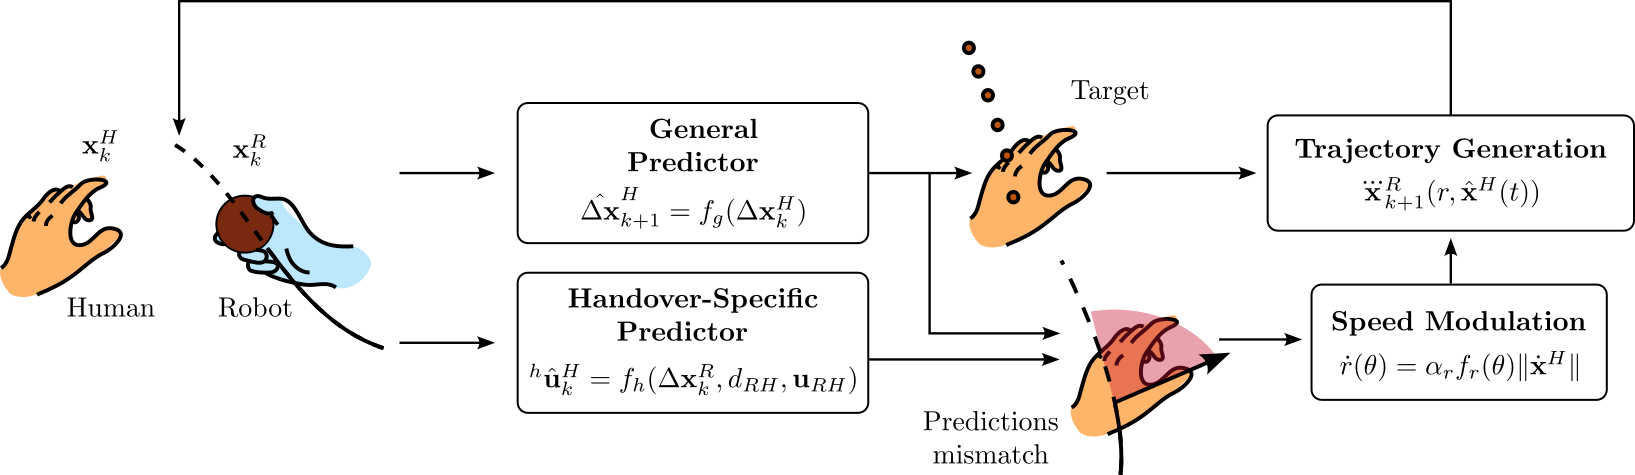
\includegraphics[width=\linewidth]{figs/big_block_diagram.png}
    \caption{Block diagram of the proposed approach. The current position of the hand of the human and the end-effector of the robot are given as input to the two predictor networks. The  output predictions on the future trajectory of the hand and the expected handover direction are then used to modulate the ratio of evolution of a dynamical system, which performs minimum-jerk tracking of the predicted trajectory.}
    \label{fig:block_diagram}
\end{figure*}

As shown in Fig. \ref{fig:block_diagram}, the neural networks output two predictions which are used to estimate whether the hand is reaching for the handover or not (i.e., whether the partner is engaged), modulating the evolution of the dynamical system.
In parallel, the predicted position of the human hand acts as a target for the online trajectory generator, which is implemented as a dynamical system performing minimum-jerk tracking.
%The following subsections describe the details of each component.

\subsection{Predictor Networks}

\noindent To detect the intent of the human partner to perform the handover action, two neural networks are trained to predict, respectively:
\begin{itemize}
    \item The short-term future trajectory ($\sim$ 0.2s) of the human hand, in general scenarios (general predictor);
    \item A vector representing the expected direction of motion for the handover (handover-specific predictor).
\end{itemize}
The second network is expected to embed a prior on where would the human hand move \textit{if it were to reach for the handover}.
As such, the detection of engagement exploits the mismatch between the predicted motion and the handover-expected motion, as shown in Fig. \ref{fig:predictor_concept}.

As we consider the case of a robot giver we simplify the notation by using the notation $R$ for the robot, implicitly in the giver's role, and $H$ for the human, implicitly in the receiver role.

\begin{figure}[h!]
    \centering
    \subfloat[]{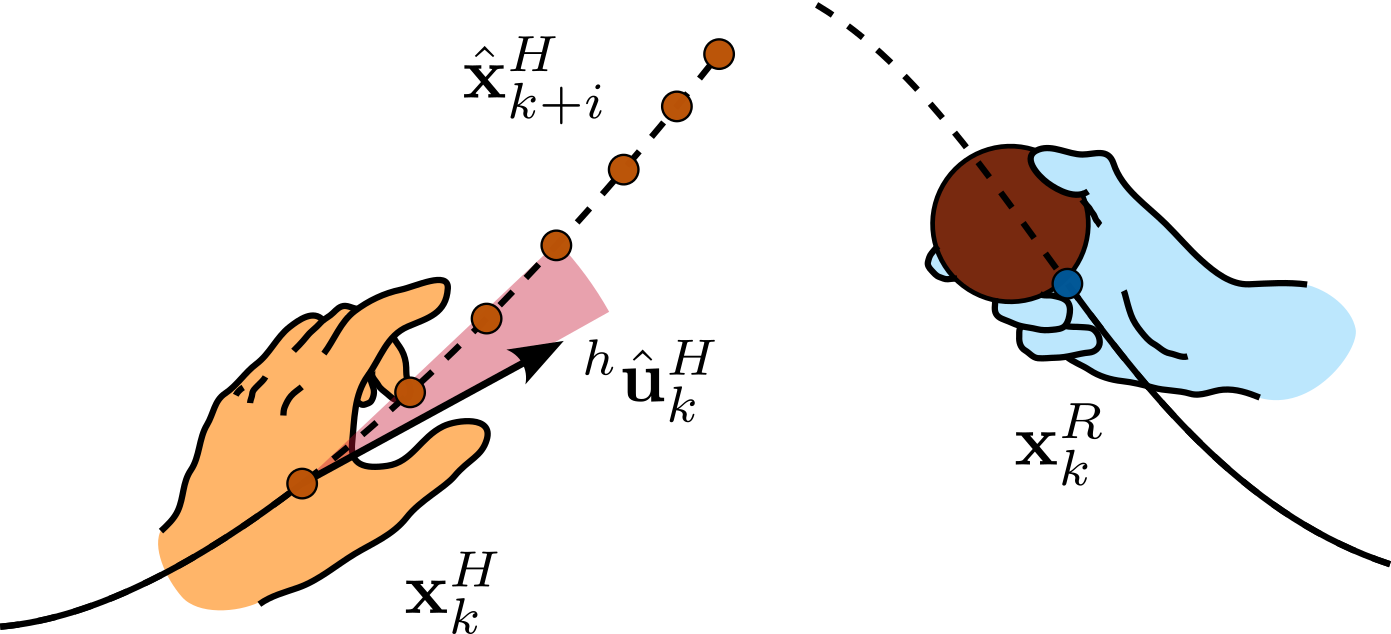
\includegraphics[width=0.48\linewidth]{figs/predictor_concept_yes_handover.png}%
    \label{fig:predictor_concept:yes_handover}}
    \hfill
    \subfloat[]{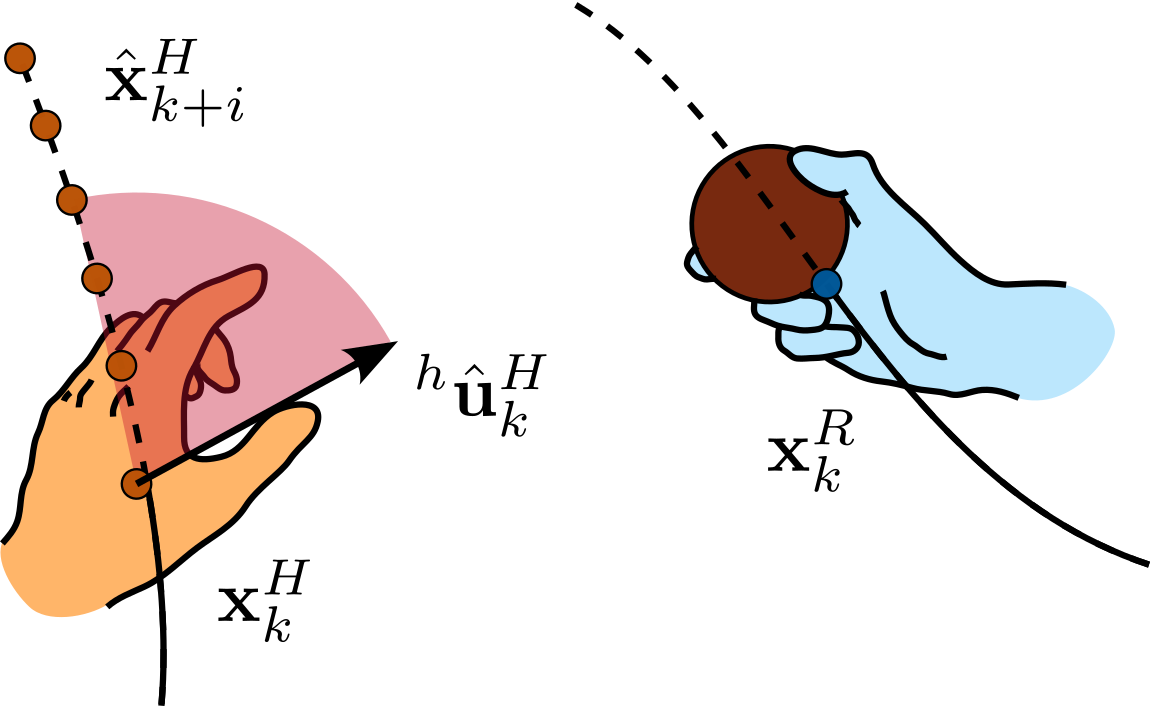
\includegraphics[width=0.4\linewidth]{figs/predictor_concept_no_handover.png}%
    \label{fig:predictor_concept:no_handover}}
    \caption{Scheme of anticipatory detection of handover intention based on two predictions, the left image represents the receiver moving for handover, the right the the opposite. Orange dots represent the predicted future trajectory of the human hand, $\hat{\x}_{k+i}^H$. The black arrow is the predicted direction of handover, ${}^h\hat{{\bm u}}_k^H$. In light red, the angular mismatch between the two (in the figure shown considering $\hat{\x}_{k+3}^H$).}
    \label{fig:predictor_concept}
\end{figure}

\subsubsection{\textcolor{black}{Datasets}}
\noindent
Already available datasets containing human-to-human handovers \cite{carfi_multi-sensor_2018}, \cite{chan_affordance_2020}, \cite{wiederhold_hoh_2023} were deemed not suitable for the purpose, as they do not contain many variations of the relative poses of the giver and the receiver and typically consider only frontal-facing interactions and/or fixed starting postures.
As such, new data were acquired using a motion capture system (Vicon Motion Systems Ltd), producing two datasets:
\begin{itemize}
    \item General Hand Motion Dataset: two persons moving freely in the motion capture volume. 5 2-minute trajectories are recorded, for a total of 10 minutes of data. The dataset contains the 3D position of the right hand of the subjects, at 100Hz.
    \item Handover Specific Dataset: a set of human-to-human handovers. The dataset contains the 3D positions of the hand of both the giver and the receiver. Different combinations of giver-receiver posture were considered (stand-stand, sit-stand, stand-sit, sit-sit), and the roles of giver and receiver were switched between participants. The relative pose (orientation, distance) of the two persons was varied freely at every interaction. The dataset is composed of the recordings of a total of 60 handover interactions, at 100Hz. A threshold of 0.03m/s on the hand speed of both the giver and the receiver was used to determine the initial cut point and the point with the smallest distance between the two hands was selected as the termination of the trajectory, restricting the recordings to the handover action. 
\end{itemize}


\subsubsection{\textcolor{black}{General Predictor}}
\noindent
The general predictor model is a machine learning model trained for the prediction of the future 3D position of the human hand.
It is implemented as a Long short-term memory (LSTM) recurrent network.
We consider to train the model to learn a prediction
\begin{equation}
    \hat{\Delta\x}_{k+1}^H = f_{g}(\Delta \x^H_k)
\end{equation}
with $\x^H_k$ the position of the human hand at step $k$, $\Delta \x^H_k = \x^H_k - \x^H_{k-1}$ the displacement of the human hand from step $k-1$ to step $k$, $\hat{\Delta\x}^H_{k+1}$ the prediction of such displacement made by the network, and $f_g$ the LSTM network.
To perform multi-step predictions, the model can be applied iteratively, using as input a prediction of the previous time step, e.g.
\begin{align}
\label{eq:model_g_iterative}
    \hat{\x}^H_{k+1} &=
    \x^H_k + f_g(\Delta\x^H_k) \nonumber\\
    \hat{\x}^H_{k+2} &=
    \hat{\x}^H_{k+1} + f_g(\hat{\Delta\x}^H_{k+1}) \nonumber \\
    & \vdots
\end{align}

The model is trained using the trajectories from the General Hand Motion Dataset.
The data are preprocessed by first filtering and then downsampling the trajectories to 30Hz.
As such, the model is trained by considering a displacement $\Delta \x^H_k$ as happening in $t_k-t_{k-1}=1/30$s.
This choice is warranted as such frequency is typically compatible with common machine learning computer vision models, that could potentially be used in place of a motion capture system \cite{lugaresi_mediapipe_2019}.
Filtering is performed using a Savitzky-Golay of order 5 with a window of 45, to remove noise in the recordings.
Three trajectories at 30Hz are generated from each original trajectory at 100Hz.

After downsampling, a data augmentation step is performed by randomly rotating, mirroring, and scaling the trajectories.
Thus, each trajectory is rotated by a random rotation matrix, mirrored around a random axis, and then scaled by a factor chosen at random in $[0.8, 1.2]$, six times per trajectory.
With this step, we aim to remove unwanted dependencies on the orientation of the specific reference frame used when recording the data.
For a similar reason, the model is trained to perform its prediction using as input a difference in positions $\Delta \x$ instead of the actual value of the position, removing the dependency of the data on the position of the reference frame during the recordings.
As such, the model is agnostic to the reference frame, making it more general for different applications. 

To train the LSTM, we consider as a loss function the Mean Square Error (MSE) in the predictions over multiple time steps, when applying the model iteratively to generate a window of $n$ predictions
\begin{equation}
    L_{g,k} = \frac{1}{n}\sum_{i=1}^n (\x^H_{k+i} - \hat{\x}^H_{k+i})^2
\end{equation}
with the predictions $\hat{\x}^H_{k+i}$ made starting from the actual position at the $k$-th time step $\x_k$ and then applying the model iteratively as in eq. \ref{eq:model_g_iterative}.
We train the model considering a window length of $n=6$.
Considering a frequency of 30Hz this corresponds to a prediction horizon of 0.2s.
Such choice comes from considering that human-to-human handovers typically have a short duration (less than 1s ) \cite{shibata_experimental_1995}, requiring adaptation on a short time scale. 
%Moreover, a long horizon typically requires more complex modeling, including multiple body parts and semantic action understanding \cite{lyu_3d_2022}, making them less appealing for online applications.

The model was implemented using PyTorch and hyperparameters optimization was performed to select the activation, number of layers, and layer sizes. Hyperparameter optimization has been performed using Bayesian Optimization with ASHA scheduling, implemented using the RayTune package.
The selected model comprises an LSTM cell with 31 hidden units, followed by two feedforward layers with 26 and 76 units respectively, both with ReLU activation, and one final output layer with linear activation. 


\subsubsection{\textcolor{black}{Handover-specific Predictor}}

\noindent
The handover-specific predictor model is a standard feedforward neural network (no recurrent connection).
The model is trained to approximate a function $f_h$ predicting 
\begin{equation}
    {}^h\hat{\bm u}^H_k = f_h(\Delta \x_k^R, d_{RH}, {\bm u}_{RH})
\end{equation}
with ${}^h{\bm u}^H_k = \Delta\x_{k+1}/\|\Delta\x_{k+1}\|$ the unit vector aligned with the next-step displacement of the human hand, ${}^h\hat{\bm u}^H_k$ its prediction, $\Delta \x_k^R = \x_k^R - \x_{k-1}^R$ the displacement of the end-effector of the robot, $d_{RH} = \|\x_k^H - \x_k^R\|$ the distance between the human hand and the end-effector, and ${\bm u}_{RH} = (\x_k^H - \x_k^R) / \|\x_k^H - \x_k^R\|$ the unit vector pointing from the human hand position to the end-effector.

The model is trained on the Handover Specific Dataset, learning to predict the direction of motion of the human hand if it were to move for a handover.
The dataset is preprocessed in the same way as for the general predictor, filtering, downsampling, and augmenting the original recordings.
The model is trained considering as a loss function the MSE between the prediction and the actual value of ${}^h{\bm u}^H_k$.
The hyperparameters of the model have been optimized with the same setup as for the LSTM general predictor model. 
The selected architecture comprises two hidden layers of 64 units each with an Exponential Linear Unit (ELU) activation function, and a final linear output layer with normalization (the output is a unit vector).

%We note that the choice of not using a recurrent network for the handover-specific predictor was due to experimenting with one, and deeming such option as not suitable.
%In fact, a recurrent network can exploit the intrinsic dynamic of human motion to make predictions (such as for the general predictor).
%When testing a recurrent handover specific model, the prediction of the future trajectory were correct when performed on the General Hand Motion dataset, even if trained only on handover trajectories.
%For the same reason, the handover specific network does not use as inputs the past positions of the human hand.

\subsection{Online Trajectory Generation}

\noindent
As explained in sec. \ref{subsec:rw:trajectory}, we propose to generate an end-effector trajectory that converges to the human hand, or, in this case, a prediction of it.
Such trajectory is generated online by a virtual dynamical system.
Specifically, we consider a time-dependent system that generates minimum-jerk tracking of a (3D position) target $\x_{des}(t)$ \cite{ghazaei_ardakani_online_2015}:

\begin{align}
    \xddd(t) =
        -\left (
            60 \frac{\eb(t)}{t_{go}^3} +
            36 \frac{\ebd(t)}{t_{go}^2} +
            9 \frac{\ebdd(t)}{t_{go}}
        \right ) + \dddot \x_{des}(t)
        \label{eq:minimum_jerk}
\end{align}

where:

\begin{itemize}
    \item  $t_{go}$ is the time left to reach the target
    \item $\x(t)$ is the current position, with components $(x,y,z)$
    \item $\eb(t) = \x(t) - \x_{des}(t)$ is the position error
\end{itemize}
As suggested in the original work \cite{ghazaei_ardakani_online_2015}, to avoid system instabilities when $t_{go}$ becomes too low, we impose a lower bound to its value
\begin{align}
    t_{go} = \begin{cases}
        t_{f}-t & t_{f}-t \geq \epsilon_{go}\\
        \epsilon_{go} & t_{f}-t < \epsilon_{go}
    \end{cases}
\end{align}
with $t_f$ the final time at which we want to reach the target and $t$ the current time, with $t_f \geq t$.
Given the considerations reported in sec. \ref{subsec:rw:trajectory}, the target $\x_{des}(t)$ is chosen as the predicted position of the human hand 6 time steps ahead, $\hat{x}^H(t_{k+6})$, obtained by applying the general predictor iteratively.
Higher-order derivatives are estimated as a filtered derivative of such prediction.

\subsection{Speed modulation}

\noindent
To adapt the robot's trajectory online, we propose slowing it down depending on the mismatch between the two predictions (general and handover-specific).
The desired behavior of the robot is to 1) stop for a mismatch above a certain (user-defined) threshold, stopping when the confidence in the handover engagement from the human is too low; 2) proceed at full speed when the mismatch is below a certain (user-defined) threshold, representing high-confidence in handover engagement; and 3) produce a smooth modulation of the speed between these two extremes.

By considering the problem of modulating the speed of the virtual dynamical system, the following subsections detail the approach proposed to obtain the behavior described.

\subsubsection{Speed of the Dynamical System}

As mentioned, in a previous work the authors employed a DMP to generate a handover trajectory and introduced custom terms to adjust its speed during a handover \cite{iori_dmp-based_2023}.
However, the dependency on \textit{ad-hoc} terms made the approach comparatively less easy to adapt, with parameters having a complex effect on the whole system's behavior.
To have a more general approach, independent of the specific dynamic of the system to modulate, we propose to modulate the evolution of a dynamical system by considering it as evolving in a virtual time $\tau$, scaled by a factor of $r$ compared to real-time, i.e. $\tau = r \cdot t$.
As an intuitive example, if we consider $r=0.5$ we would like our system to move at half the speed of the original one.
To develop such an approach let's consider a general dynamical system in the form
\begin{equation}
    \frac{d \y}{d\tau} = f(\y, u, \tau)
\end{equation}
with $\y = (\x, \frac{d\x}{d \tau}, \frac{d^2\x}{d \tau^2}, ...)$.
Applying the chain rule for derivatives (considering that $r$ is set independently from $t$), we get
\begin{equation}
     \xd \triangleq \frac{d\x}{d t} = \frac{d\x}{d \tau} \frac{d\tau}{d t} = r \frac{d\x}{d \tau} 
\end{equation}
and, generally
\begin{equation}
\label{eq:general_scaling_law}
     \frac{d^n\x}{d t^n} = r^n \frac{d\x}{d \tau^n} 
\end{equation}
Practically, this produces a scaling of the velocity and all higher-order derivatives of the dynamical system, modulating the speed of evolution without ad-hoc terms.
As such, adjusting $r$ in $[0,1]$ will thus modulate the system between null speed and full speed of the original system. 
It is noted that $r$ should be continuous, to avoid discontinuities in velocity, acceleration, and so on, as per (\ref{eq:general_scaling_law}).
Finally, it is noted that $t_{go}$ is replaced by $\tau_{go}$ when applying the method to the minimum jerk dynamical system in (\ref{eq:minimum_jerk}).


\subsubsection{From Predictions to Speed Modulation}

The previous section introduced a method to modulate the speed of a dynamical system, with the desiderata that this should happen according to a "mismatch" between the general and handover-specific predictions, representing the engagement of the human in the handover.
To do so, we consider modulating the value of $r$ as a function of the angle $\theta$ between the two predicted directions of motion
\begin{equation}
    \theta = \arctan2(\hat{\bm u}_{k}^H \cdot \hat{\bm u}_{k,k+6}^H, \hat{\bm u}_{k}^H \times \hat{\bm u}_{k,k+6}^H)
\end{equation}
with $\hat{\bm u}_{k,k+6}^H$ a unit vector pointing from the current position of the human hand to its predicted position after 6 time steps.
as represented in Fig. \ref{fig:predictor_concept}.
While we could directly modulate the value of $r$ in using $\theta$, a notable edge case arises if we consider a moment where the hand is not moving, where we expect $\hat{\bm u}_{k,k+6}^H$ to not be particularly informative about the future.
In such case, should the human taker, after reaching forward, wait for the object to be delivered, the robot should perform the handover.
However, should the human partner have stopped their hand due to an interruption (or should the partner not yet engage in the handover), the robot should not move.
%Indeed, if the hand is not moving it could be either because the partner already reached forward, and is waiting for the robot to deliver the object, or because an interruption occurred and the partner stopped (in which case the robot should not move).
%In this case, the partner could be waiting for the object to be delivered, after reaching forward, and the robot should perform the handover.
%Alternatively, the partner may have removed their hand from the interaction, or not even engaged in it yet, and the robot should not move. 
To address this ambiguity, we apply a first-order dynamic to the ratio $r$ and make it dependent on the velocity of the hand
\begin{align}
    \dot r(\theta) = \alpha_r f_{r}(\theta) \|\xd^H\|
\end{align}
where $\alpha_r$ is a parameter of the system, $\|\xd^H\|$ the norm of the velocity of the human hand, and
\begin{equation}
    f_r(\theta) = 1-2\left( \frac{1}{1+e^{\sigma_{s}(\sigma_{o}-\theta)}} + \frac{1}{1+e^{\sigma_{s}(\theta+\sigma_{o})}} \right)
\label{eq:ratio_function}
\end{equation}
is a "hat-shaped" function, obtained as the combination of two sigmoids.
Thus, $\sigma_o$ and $\sigma_s$ are parameters controlling the offset and steepness of the sigmoids, respectively, as shown in Fig \ref{fig:ratio_function}.

\begin{figure}
  \begin{minipage}[c]{0.48\linewidth}
    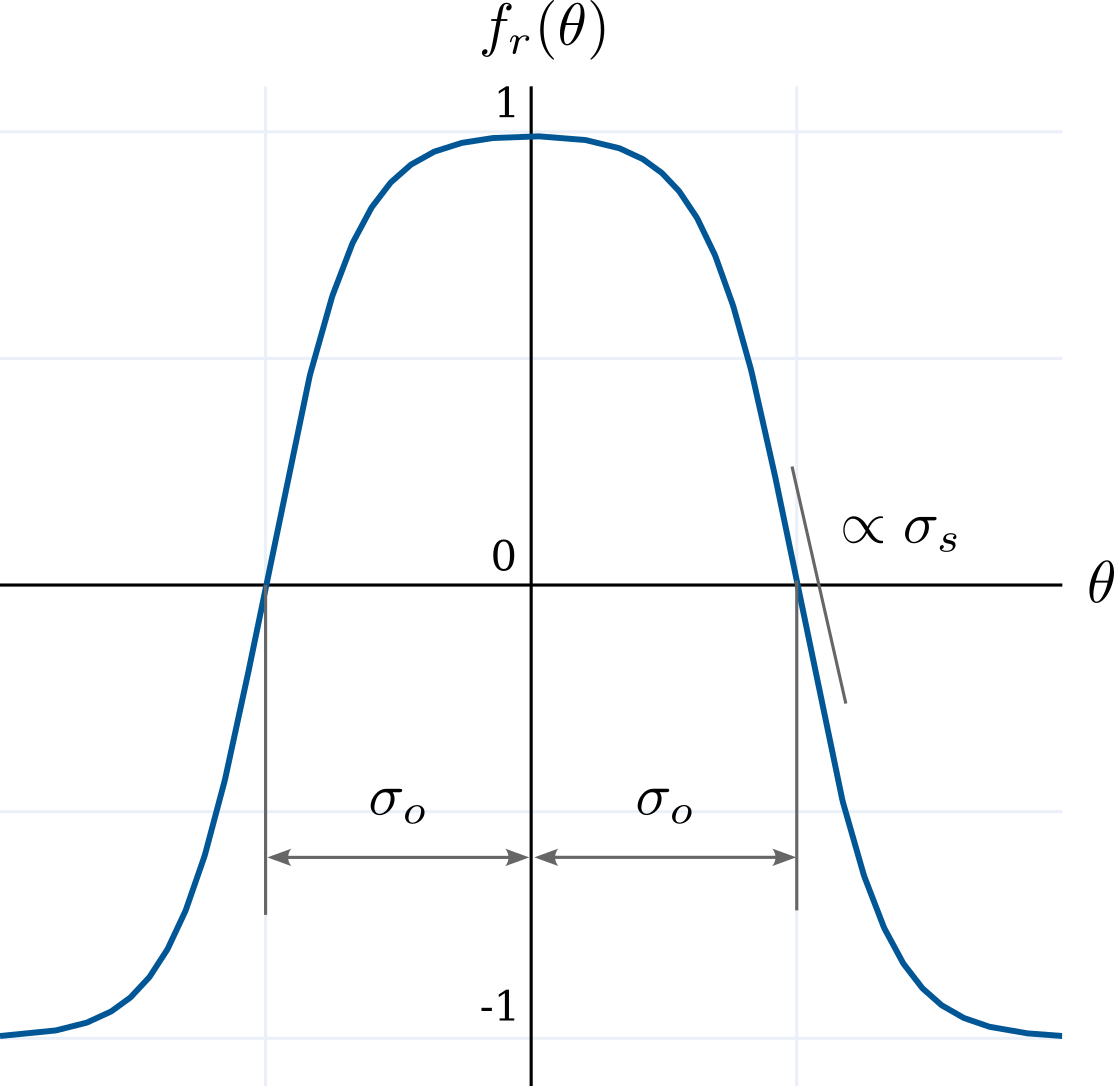
\includegraphics[width=1.0\linewidth]{figs/ratio_function.png}
  \end{minipage}\hfill
  \begin{minipage}[c]{0.5\linewidth}
    \caption{Function $f_r(\theta)$, controlling the effect of the misalignment angle, $\theta$, on the acceleration or deceleration of the system between none and full speed. $\sigma_o$ defines the range in which the robot should accelerate towards full speed of its trajectory, i.e. "engage" in the handover. $\sigma_s$ controls the steepness of this change.}
    \label{fig:ratio_function}
  \end{minipage}
\end{figure}

%\begin{figure}[h!]
%   \centering 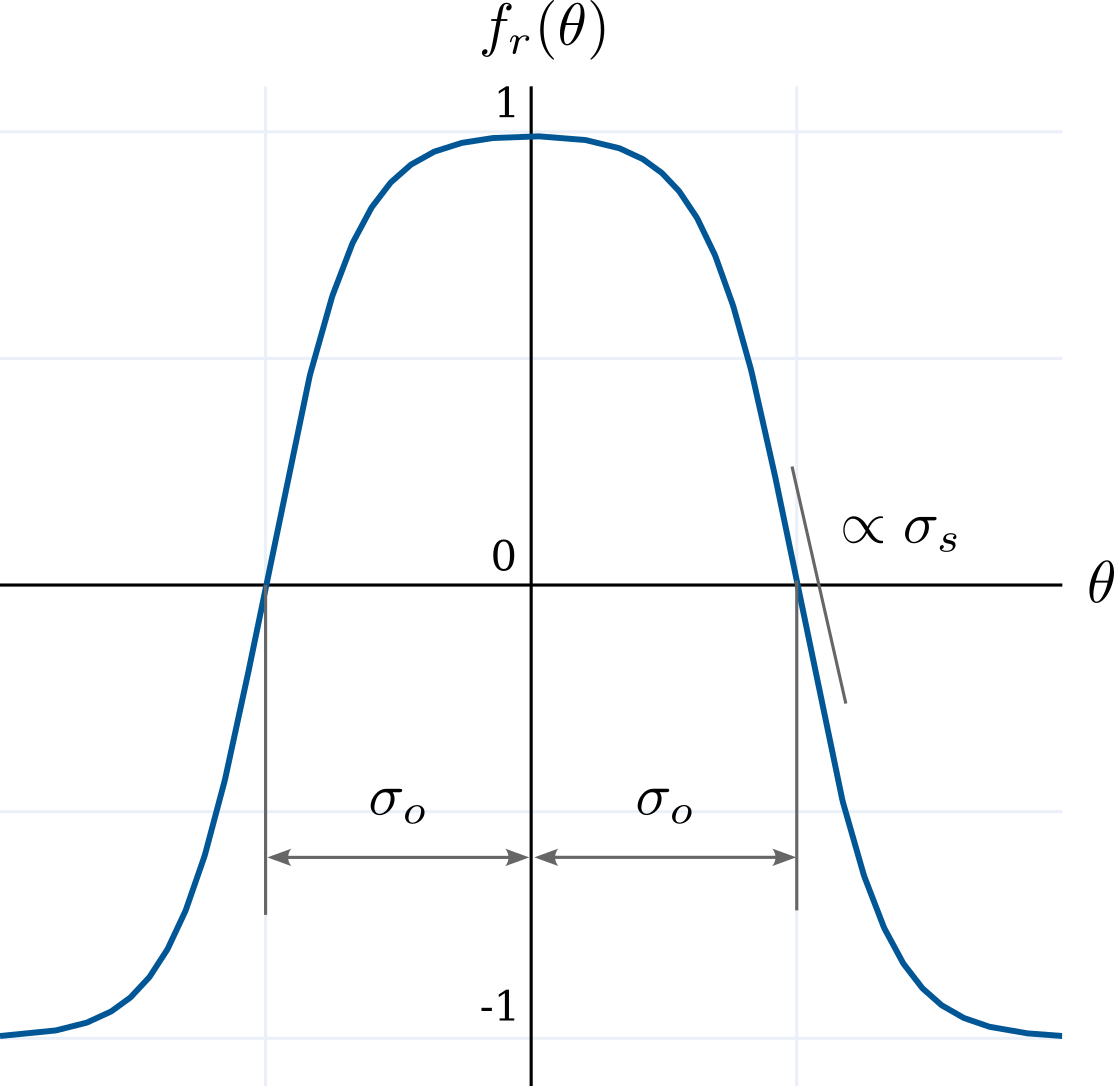
\includegraphics[width=0.5\linewidth]{figs/ratio_function.png}
%    \caption{Function $f_r(\theta)$, controlling the effect of the misalignment angle, $\theta$, on the acceleration or deceleration of the system between none and full speed. $\sigma_o$ defines the range in which the robot should accelerate towards full speed of its trajectory, i.e. "engage" in the handover. $\sigma_s$ controls the steepness of this change.}
%    \label{fig:ratio_function}
%\end{figure}

This choice of how to modulate $\dot r$ provides interpretable parameters to control the behavior of the system, along with a "memory" effect that preserves the value of $r$ when the hand is not moving.
Considering Eq. \ref{eq:ratio_function}, the value of the rate of change $\dot r$ is proportional to the absolute speed of the human hand $\|\xd^H\|$, with $\alpha_r$ setting the overall scale. 

%\textcolor{teal}{should we mention something about humans adjusting to the speed of the partner? \cite{controzzi_humans_2018})}.

The parameter $\sigma_o$ defines the range of alignment $\theta$ in which the system should increase the speed of execution ($\dot r>0$).
$\sigma_o$ controls the range of mismatch between the two predictions for which we still desire the robot to keep engaging in the interaction.
The parameter $\sigma_s$ defines the steepness of the change, or how abrupt should the system transition between slowing down or speeding up.

\subsubsection{Practical Considerations}
\label{subsec:speed_modulation:practical_considerations}

Using the method introduced in this section, a mismatch in the predictions is used to scale the speed of the virtual dynamical system that generates the trajectory.
To improve the practicality of the system, both $r$ and $\dot r$ are clipped, to $[0,1]$ and [-$\dot r_{max}$, $\dot r_{max}$], respectively.
Clipping $r$ ensures that the virtual dynamical system will never evolve faster then the "baseline" system, with $r=1$.
As such, a positive or negative value of $\dot r$ determines whether the robot is engaging or disengaging from interacting, respectively.
Clipping $\dot r$ sets a limit to how fast the system can react, to avoid excessive accelerations or decelerations.

Finally, the value of $r$ at the start of the interaction, $r_0$, can be set depending on the intended application: an initial value of 0 would make the robot wait for motions of the human that can be interpreted as handover, which would then raise the ratio and speed up the robot. 
As the initial value is set closer to 1, the robot starts the interaction with the full speed of the dynamical system.
Thus, it slows down only as a reaction to motions that are not interpreted as handover.

\section{Experimental Evaluation}

\noindent
We consider three different scenarios for an experimental assessment of AntIP:
\subsubsection{Standard Handover}
Under normal conditions (no perturbation), how does the anticipatory modulation impact the coordination and completion time of the handover?
\subsubsection{Delayed Handover}
Can the system prevent the robot from unsafely moving towards the human, if the robot starts executing the handover before the human (e.g., such as when the human partner is distracted)?
\subsubsection{General Perturbations}
Can the system reliably adapt the robot's speed under general and unpredictable perturbations?

%We note that this set of tests is meant as a first general assessment of the proposed system under a variety of scenarios and is not intended to evaluate human perception and behavior when interacting with the proposed system. 

\subsection{Setup}

\noindent
The robotic setup used to perform the robotic handover consists of a Universal Robots UR5 CB-series manipulator equipped with IH2 Azzurra hand (Prensilia SRL) \cite{cipriani_smarthand_2011}.
To track the motion of the human hand a Vicon motion capture system with 6 Bonita cameras (Vicon Ltd) is used.
Markers are placed on the back of the hand of the subjects, and additional markers are also placed on the Azzurra hand.
A speaker is used to give the participants an auditory "Go" signal, corresponding to the start of the handover interaction.
The system is controlled via ROS, implementing both the predictors and the trajectory generation as ROS nodes and using a state machine to execute the scenarios.
When the robot is triggered to start the handover, the virtual dynamical system is initialized in the current end-effector state, and online trajectory generation is performed as presented, tracking the predicted trajectory of the human hand as described above.
To perform a full interaction, a simple release controller is also implemented.
The controller triggers a "soft" stop of the dynamical system when the distance between the hands falls below a fixed threshold of 20cm.
This is performed by setting the target of the minimum-jerk tracking to its own current position.
Then, after a fixed time of 0.5s, the Azzurra hand is triggered to open to release the object.

As the Vicon system is set to run at 100Hz, its output is first filtered with a second-order linear low pass filter with a cutoff at 40Hz, and the predictions with the two models are computed at a rate of 30Hz, using at each time step the last available positions of the human hand and robot.
A third-order linear low pass filter with a cutoff at 14Hz is used to compute filtered derivatives from the output of the general predictor.

In each execution, we record:
\begin{itemize}
    \item The trajectory of the human hand;
    \item The trajectory of the robot hand;
    \item The predictions made by the two networks;
    \item The value of the ratio $r(t)$;
    \item The RGB stream from an Intel\textsuperscript{\textregistered} RealSense\textsuperscript{\textregistered} D435 camera.
\end{itemize}

Three sets of parameters for the system are considered: A non-reactive set, NR, where the minimum-jerk tracking is left to evolve freely with no adaptation (ratio $r$ fixed to 1); and two reactive sets, R0 and R1, where $r$ is controlled as proposed, and where the initial value $r_0$ it set to 0 and 1, respectively.
The value of the parameters of these sets are reported in Table \ref{tab:parameters_set}

\begin{table}[h!]
    \caption{Set of controller parameters}
    \label{tab:DMP_params}
    \begin{center}
        \begin{tabular}{l|rrrrrrr}
            & $t_{go}(0)$ & $\epsilon_{go}$ & $\alpha_r$ & $\sigma_o$ & $\sigma_s$ & $r_0$ & $\dot{r}_{max}$\\
            \midrule
            NR & 2s & 0.2s & - & - & - & - & -\\
            R0 & 2s & 0.2s & 10.0 & 0.55& 12.0 & 0.0 & 25\\
            R1 & 2s & 0.2s & 10.0 & 0.55& 12.0 & 1.0 & 25\\
        \end{tabular}
    \end{center}
    \label{tab:parameters_set}
\end{table}
%These values were picked during preliminary trials when setting up the whole pipeline for the experiments.
%, and do not necessarily represent an optimal choice.
To avoid practical safety issues, due to the robot moving towards the human before they're aware, only the R0 set of parameters is applied in the \textit{Delayed Handover} scenario; this is a more conservative configuration in which the system does not assume that the human is engaged from the start of the interaction.
For similar safety reasons, especially considering reaction times and the variability introduced by perturbations such as throwing an object, we employ only R0 in the \textit{General Perturbation} scenario.
We note, however, that the system's anticipatory reaction (i.e. $\dot r$) to the human motion is not influenced by the choice of $r_0$, providing an evaluation of the system response to perturbations.

\subsection{Protocol}
\label{subsec:protocol}

\noindent
In all three scenarios, the robot hands over an empty 0.5$l$ bottle to the human partner, and the human is tasked to engage in the handover interaction upon hearing the "Go" signal from the speaker. 

The \textit{Standard Handover} and \textit{Delayed Handover} scenarios were tested in the same experimental session.
In the \textit{Standard Handover} the speaker gives the "Go" signal as soon as the robot starts the handover.
Differently, when performing a \textit{Delayed Handover}, the "Go" signal is given to the participant with a random delay uniformly sampled in the range $[0.5, 1.5]s$. 
As mentioned, only the R0 set of parameters is tested in this last setting, while all three are tested in the condition of \textit{Standard Handover}.
As such, a total of 40 interactions per participant are performed, 10 per each combination of parameter sets and scenarios.
Of these 10 interactions per set of parameters, 5 are performed with the participant standing, and 5 with the participant sitting.
Before the start of the experiment, participants performed a few ($5$) interactions with each of the three sets of parameters, to get used to the system.

The \textit{General Perturbations} scenario is conducted to test the behavior of the system in edge cases.
%Similarly to the \textit{Delayed Handover} scenario, all the interactions were performed with the R0 set of parameters.
During the entirety of each of these interactions, the robot is engaged in the execution of the handover.
As such, if the trajectory is not slowed by the proposed system, the robot performs minimum-jerk tracking of the predicted pose of the human hand, possibly invading the space around the human.
To avoid significant safety issues these interactions are performed with the robot out of reach of the participant's head and torso.

%%%
The interactions recorded are composed by:
\begin{itemize}
    \item 2 interactions where the subject "fakes" and gets back the hand, as in the practical joke described in Sec. \ref{sec:introduction}, before reaching again for a handover (A); 
    \item 2 interactions where the robot is engaged in the handover and the subject waves their hand before reaching, to further test the capability of waiting for a handover motion (B);
    \item 2 interactions where the arm of the subject is slapped by another subject during the handover (C);
    \item 6 interactions where, during the handover, the subject is thrown:
    \begin{itemize}
        \item A light plastic toy (D);
        \item A basketball (E);
        \item A large beanbag (F).
    \end{itemize}
    %\item 2 interactions where the subject has to catch a basketball thrown to them during the handover (E);
    %\item 2 interactions where a large beanbag is thrown at the subject during the handover (F).
\end{itemize}
These sets of interactions are meant to produce adversarial or unpredictable perturbations during the handover.

\section{Results}

\noindent
All the data recorded during the experimental evaluation are available as supplementary material as \texttt{.rosbag} files, including the synchronized RGB camera feedback.
After the recording, the original trajectories were filtered with a Savitzky-Golay filter (window=11, order=3) to reduce the noise from the motion capture system and to compute filtered derivatives.



\subsection{Standard and Delayed handovers}

\noindent
To qualitatively assess whether the proposed method could coordinate the robot in a standard handover scenario, we consider the plots shown in Fig. \ref{fig:std:dist_vs} and \ref{fig:std:norm_speed}.
A threshold of 0.3s was applied to discard trajectories where the hand is lost for too long by the motion capture system, as a consequence of occlusion.
The trajectories analyzed are 25 (NR), 30 (R0), 28 (R1), 26 (R0, Delayed).
Fig. \ref{fig:std:dist_vs} shows a comparison of the evolution over time of the normalized distances from the final handover location of the human and the robot, plotted against each other.
The values in the plot correspond to $1-\frac{\| \x(t) - \x(t_f) \|}{\| \x(0)-\x(t_f) \|} $, computed both for the human and the robot, with $t_f$ being the time after which the two meet at the final location from the start of the interaction.
The interaction starts in $(0,0)$ and evolves to $(1,1)$ as both agents reach the handover location.
The diagonal (shown dashed) represents a hypothetical perfectly coordinated handover, with both agents covering the same relative distance at the same time.
This approach draws inspiration from neuroscience literature, with similar assessments of motor coordination and force during grasp across different conditions \cite{flanagan_coupling_1993} \cite{gordon_fingertip_1999} \cite{cipriani_humans_2014}, including object handover \cite{controzzi_humans_2018}.
Fig. \ref{fig:std:norm_speed} shows the evolution of the (normalized) absolute speed in the \textit{Standard Handover}, represented as the mean and shaded confidence bounds.
The same graph is not reported for the \textit{Delayed Handover} scenario because the trajectories are purposefully misaligned in time, due to the random delay in the scenario.

Table \ref{tab:std:coordination_delay} shows the time differences between the robot and the human in completing percentages (25, 50, and 75 \%) of the handover trajectory, which similarly can be taken as a metric of coordination.
Positive values correspond to the robot covering the corresponding percentage before the human, represented by the trajectories in Fig. \ref{fig:std:dist_vs} being above the diagonal, and negative values vice versa.
No statistically significant difference ($p>0.05$) is found between the values produced by the parameters pairs (NR, R1) and (R0, R0-Delayed), for all percentages.
On the other hand, a statistically significant difference ($p<0.001$) is found between all other reciprocal pairs, for all percentages.
Significance has been evaluated using a Kruskal-Wallis non-parametric test.

\begin{table}[h!]
\scriptsize
    \begin{center}
        \begin{tabular}{l|cccc}
        & NR & R0 & R1 & R0-Delayed \\
        &&&&\\
        
        25\% & $ 0.077_{-0.058}^{+0.088}$ & $-0.496_{-0.031}^{+0.034}$ & $ 0.025_{-0.011}^{+0.011}$ & $-0.577_{-0.137}^{+0.119}$ \\
        &&&&\\
        
        50\% & $ 0.008_{-0.060}^{+0.091}$ & $-0.532_{-0.044}^{+0.044}$ & $-0.045_{-0.014}^{+0.014}$ & $-0.708_{-0.262}^{+0.208}$ \\
        &&&&\\
        
        75\% & $-0.052_{-0.059}^{+0.086}$ & $-0.521_{-0.053}^{+0.048}$ & $-0.116_{-0.023}^{+0.025}$ & $-0.785_{-0.364}^{+0.301}$ \\

     
        \end{tabular}
    \end{center}
    \caption{Mean time differences [$s$] and confidence bounds in covering the 25\%, 50\%, and 75\% of the handover trajectory between the robot and the human. Positive values show that the robot covered first the corresponding percentage, and negative values vice versa.}
    \label{tab:std:coordination_delay}
\end{table}


Table \ref{tab:std:task_completion_time} reports the task completion time, calculated from the "Go" signal given to the human to when the Azzurra hand is commanded to open, thus removing the random delay in the \textit{Delayed Handover} scenario.
No statistically significant difference ($p>0.05$) is found between the pairs (NR, R1) and (R0, R0-Delayed), while a statistically significant difference ($p<0.001$) is found between all other pairs. Values were compared with a Kruskal-Wallis non-parametric test.

\begin{figure}[]
    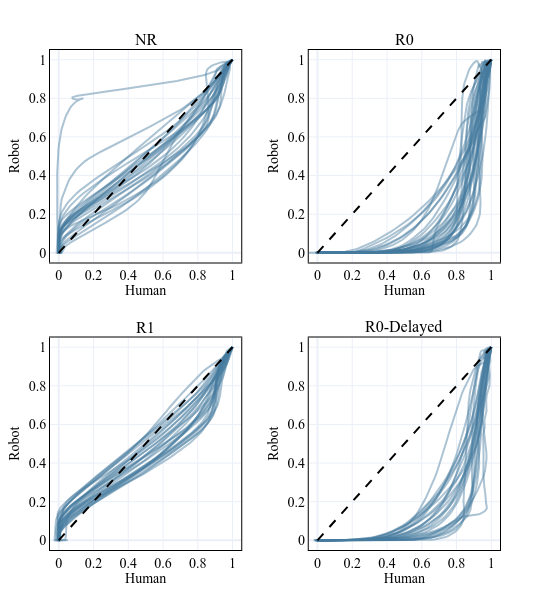
\includegraphics[width=\linewidth]{figs/std_dist_vs.png}
    \caption {Comparison of the (inverted) normalized distance from the final handover location. The value plotted is $1-\frac{d}{d_0}$. For each graph, the $x$-axis corresponds to the human and the $y$-axis to the robot.
    At the start of the interaction both agents are in 0.0, and 1.0 corresponds to reaching the final position. The dashed diagonal line represents a hypothetical interaction with each agent covering the same relative distance at every step.}
    \label{fig:std:dist_vs}
\end{figure}

\begin{figure*}[t]
    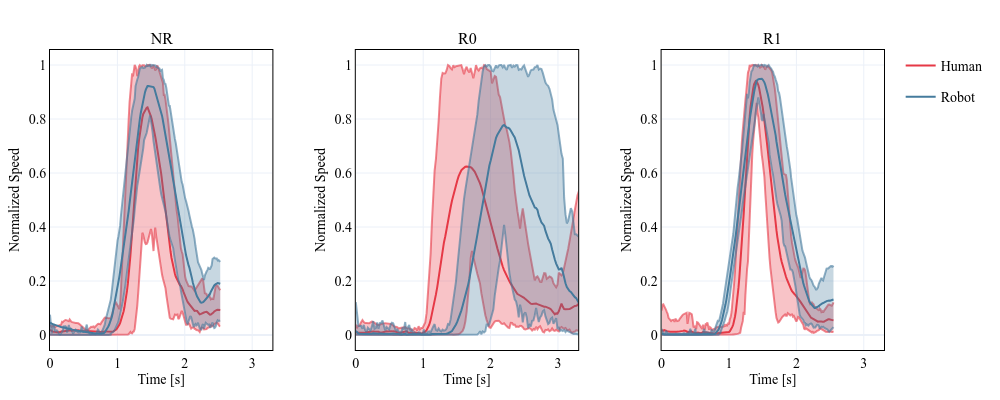
\includegraphics[width=\textwidth]{figs/std_norm_speed_mean_confidence.png}
    \caption {Evolution in time of the normalized absolute speed of the subject and the robot in the straight handover scenario.
    The solid line represents the mean, and the shaded area corresponds to the 5-95\% data percentiles.}
    \label{fig:std:norm_speed}
\end{figure*}


\begin{table}[h!]
    \begin{center}
        \begin{tabular}{l|cc}
            & Mean ($^{+95\%}_{-5\%}$ CI) [s] & 5-95\% Percentiles [s] \\
            &&\\
            NR & $2.30^{+0.04}_{-0.04}$ & 2.13-2.48 \\
            &&\\
            R0 & $3.04^{+0.10}_{-0.10}$ & 2.59-3.59 \\
            &&\\
            R1 & $2.31^{+0.04}_{-0.04}$ & 2.14-2.47 \\
            &&\\
            R0-Delayed & $3.39^{+0.49}_{-0.37}$ & 2.60-5.32 \\
            
        \end{tabular}
    \end{center}
    \caption{Mean task completion time in the straight handover scenarios; 5-95\% confidence intervals on the mean and 5-95\% percentiles are also reported.}
    \label{tab:std:task_completion_time}
\end{table}

\subsection{General Perturbations}

\begin{figure*}[h!]
    \centering
    \subfloat[\footnotesize Interaction A.1. The participant takes back the hand after reaching out (as per example in Sec. \ref{sec:introduction}), before reaching again for the handover. \label{fig:perturbed:B.2}]{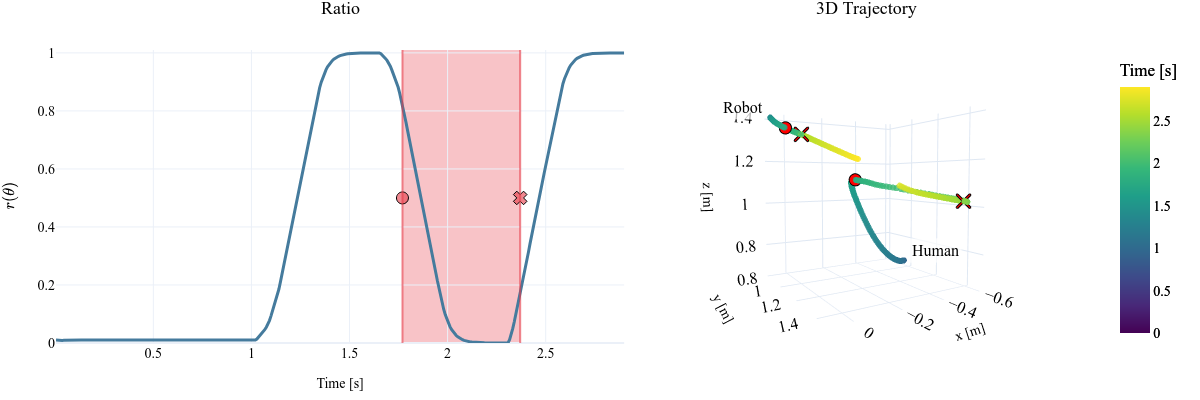
\includegraphics[width=0.7\textwidth]{figs/perturbed_ratio_3d/A.1.png}}
    \\
    \subfloat[\footnotesize Interaction B.2. The participant waves their hand before reaching for the handover. \label{fig:perturbed:B.2}]{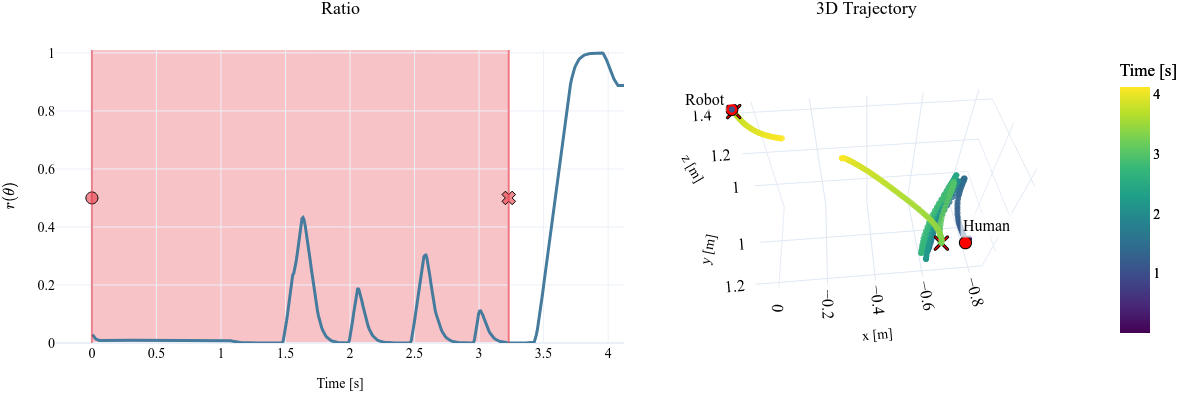
\includegraphics[width=0.7\textwidth]{figs/perturbed_ratio_3d/B.2.png}}
    \\
    \subfloat[\footnotesize Interaction C.2. The participant's arm is slapped. \label{fig:perturbed:2}]{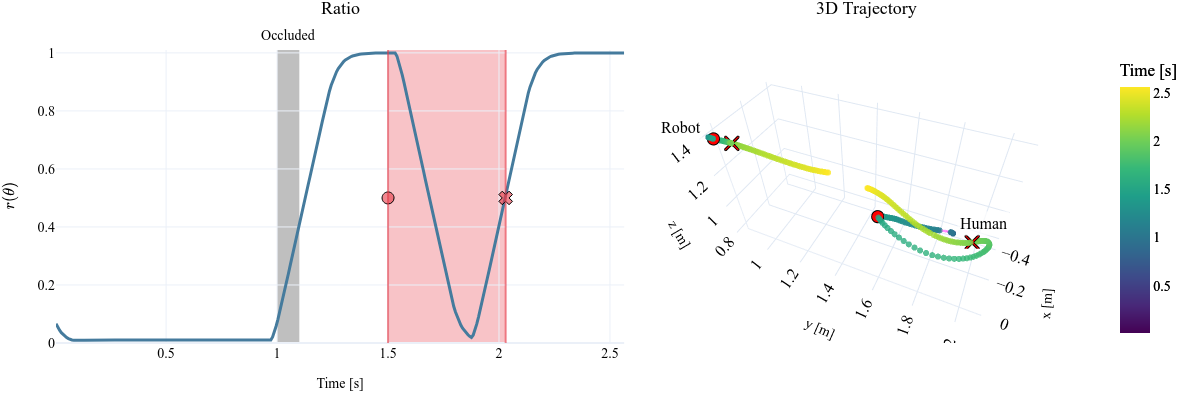
\includegraphics[width=0.7\textwidth]{figs/perturbed_ratio_3d/C.2.png}}
    \\
    \subfloat[\footnotesize Interaction D.1. The participant is thrown a light plastic toy. \label{fig:perturbed:3}]{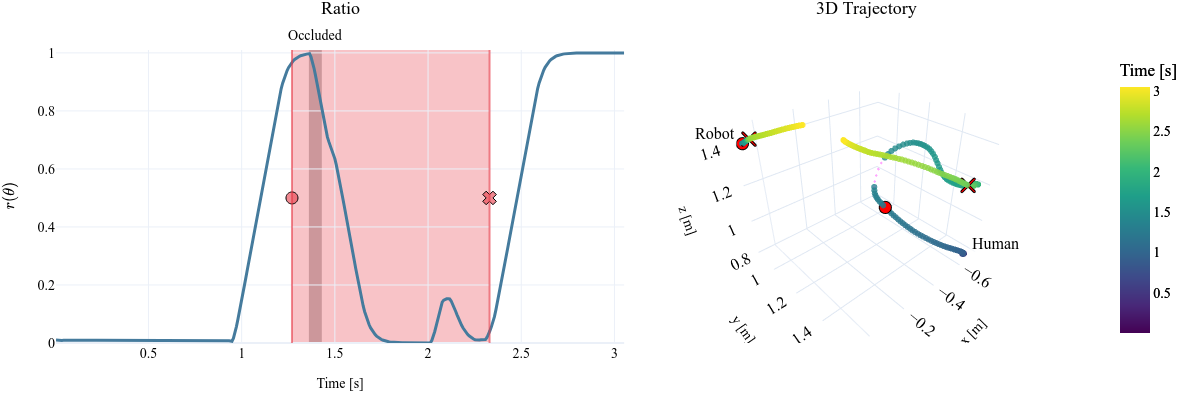
\includegraphics[width=0.7\textwidth]{figs/perturbed_ratio_3d/D.1.png}}
    
    \hfill

    \caption{Evolution of the ratio and 3D trajectory during four interactions (A.1, B.2, C.2, D.1) in the General Perturbation scenario.
    The red shaded area denotes the time between the start and the end of the perturbation.
    The red circle and cross show the points selected as the start and the end of the perturbation, respectively.
    The color scale denotes corresponding time steps in the two trajectories, with points recorded at the same time as the same color.
    Finally, the gray shaded area denotes part of the interaction where the human hand was occluded; the 3D plot shows a hypothetical interpolated trajectory with small pink markers.
    Interactive 3D plots, and the associated video of the interaction, are available at \url{https://fraiori0.github.io/antip-handover/}.
    }
    \label{fig:perturbed:all}
\end{figure*}

\noindent
A qualitative assessment of a wide range of handover interactions including unstructured perturbations is considered.
To assess the behavior of the system in these scenarios, Fig. \ref{fig:perturbed:all} reports the evolution in time of the ratio $r(\theta)$ during three example interactions, along with the 3D trajectory of the robot and the human during the handover.
In Fig. \ref{fig:perturbed:all}, highlighted in red is the time during which the perturbation lasts (on the ratio plot, right) and the initial and final points that were selected as the start and end of the perturbation (on the 3D trajectory, left); the figure also shows when the hand was occluded to the motion capture.
The expected behavior of the system is to predict (the lack of) human engagement during the perturbation, modulate the trajectory accordingly by slowing down, and then when the human partner re-engages execute the handover.
The same plots but for all interactions in the \textit{General Perturbations} scenario are available as supplementary material, and interactive plots and videos from the interactions can be seen at \url{https://fraiori0.github.io/antip-handover/}.

\section{Discussion}
\label{sec:discussion}

\subsection{Standard and Delayed handovers}

\noindent
The scenario of \textit{Standard Handover} is set up as an idealized handover, commonly discussed in the literature.
Thus, should both agents start at the same time, fully engaging in the interaction, the agents would be coordinated, covering similar relative distances over time.
This can be observed from Fig. \ref{fig:std:dist_vs} by considering the plots relative to the NR and R1 sets of parameters: the resulting curves are both mostly clustered around the idealized coordination line.
By considering the very first part of the curves after the origin, it can also be noticed how the robot actually engages slightly sooner in the interaction.
This can be reasonably expected due to a lag in the human recognizing and reacting to the auditory signal; such lag is eventually recovered by the human, who starts then slowing down typically slightly sooner than the robot, as can be observed in Fig. \ref{fig:std:norm_speed}.
Conversely, by considering the R0 and R0-Delayed plots in Fig. \ref{fig:std:dist_vs}, it can be noted that the robot never starts moving before the human is engaged in the handover, corresponding to a horizontal tangent of the curves in the origin.
For this reason, for both the \textit{Standard} and \textit{Delayed} scenarios, the resulting curves for the respective R0 and R0-Delayed parameter settings follow similar profiles, as even with the delay the robot follows the human. 
The values reported in  Table \ref{tab:std:coordination_delay} support a similar perspective, showing that when both the human and the robot start fully engaged (NR and R1 parameters) they have little mean relative delay ($\leq 0.116 s$) in completing the same relative amount of the trajectory.
The similarity in these values between NR and R1 (along with the absence of any statistically significant difference), suggests that the reactive modulation does not interfere with the coordination in the joint action when no perturbation is present and the robot starts fully engaged (i.e., with $r_0=1.0$), producing a coordinated handover.

When the task completion time in Table \ref{tab:std:task_completion_time} is considered, since no statistical significance was found between the NR and R1 parameter settings, it can be concluded that the proposed method can produce adaptive behavior with comparable task performance, given that both agents initiate the motion simultaneously. 
Expectedly, the same parameter settings for R0 and R0-Delayed interactions produce higher task completion times as the robot now has to wait until human engagement is detected for enough time to increase the ratio before the trajectory can start to evolve.
Practically, this results in waiting for the human to engage first, as visible in Figs. \ref{fig:std:dist_vs}-\ref{fig:std:norm_speed}.
Importantly, since there is no statically significant difference between R0 and R0-Delayed, the resulting behaviors are as intended.

As a qualitative metric of the ability of the method to produce a standard handover, Fig. \ref{fig:std:norm_speed} reports the speed profiles of the human and the robot during the \textit{Straight Handover} scenario.
Considering the speed profiles reported by Shibata et al. \cite{shibata_experimental_1995}, where frontal human-to-human unperturbed handovers were analyzed, observing minimum-jerk speed profiles that are mostly overlapped (with a shift indicating that one agent engages first in the interactions, and the other follows), the profiles are comparable.
%Curiously, the set of parameters R1 seems to produce more aligned interactions, when NR should be expected to have comparable performances in the Straight handover scenario.

While the R0 parameter setting produces a higher task completion time, the practical benefit of the practical benefit of the robot waiting for the human to engage can be desirable, as exemplified in the \textit{Delayed Handover} interactions.
In scenarios where a high-level controller could start the execution of the handover while the human is distracted, the conservative settings of R0 provide an additional, robust, low-level safety feature.
On the other hand, should this behavior not be needed, less conservative parameter settings (such as R1) could be selected, thus not compromising task completion time in straightforward interactions, while still being able to adapt to perturbations that might arise at later stages of the interaction.

\subsection{General perturbations}

\noindent
By considering the plots of Fig. \ref{fig:perturbed:all}, it can be qualitatively assessed how the anticipatory adaptation affects the trajectory during a perturbed handover.
The proposed approach can be observed to produce a smoothed and lagged profile of the ratio $r$, which can be attributed to the first order dynamics and clipped derivative of the ratio.
We note that delayed reactions can produce more pleasurable interactions during robot-human handovers, as shown in \cite{pan_fast_2019}.
As desirable, the ratio reliably reacts to the perturbation, slowing down and speeding up the dynamical system generating the trajectory.
Using the set of parameters R0, the robot follows the partner in the handover, slowing and stopping the trajectory as a reaction to perturbation.
As a consequence, the robot covers most of the trajectory after of the perturbation.
This can be noticed in the 3D plots of Fig. \ref{fig:perturbed:all}, where points of the same color represents where the human and the robot were at the same time, and the red and green markers those selected as start and end of the perturbation.

Figs. \ref{fig:perturbed:A_B}, \ref{fig:perturbed:C_D}, and \ref{fig:perturbed:E_F} shows the same plots for all the interactions of the General Perturbation scenario.
It is noted that, in some of these trajectories, the hand is occluded for a significant amount of time.
Nonetheless, it can be observed from the recordings how the system is able to produce what can be considered an acceptable behavior of the system.
This can be attributed to the first-order dynamics of the system, producing a gentle degradation of the performances of the system in case of occlusions. 
If some part of the trajectory is visible (especially at the start of the perturbation) and is correctly interpreted as not compatible with the handover the system is slowed down.
Once the hand disappears due to occlusion the system maintains its current value of the ratio $r$, until new, non-occluded data can affect its behavior again.
\\

\noindent
As noted, the choice of the initial value of ratio ($r_0$) can happen according to application-specific requirements.
As an example, choosing $r_0=0$ would be suited to applications where there's uncertainty on whether the human is engaged in the handover from the start of the interaction.
On the other hand, $r_0=1$ could be adopted in systems that are more conservative in deciding when to start the interaction, where the robot should engage right from the start.
Finally, the other parameters of $f_r(\theta)$ can be used to fine-tune the response to the misalignment in the two predictions, providing interpretable values to set the response of the system to perturbations. 


\section{Conclusions}
\label{sec:conclusions}

\noindent
This work proposed an approach for the online adaptation of trajectories for robot-to-human handovers under perturbations, inspired by the concept of anticipatory control.
The main benefits of the approach can be seen in terms of
\begin{itemize}
	\item Interpretability: by providing interpretable parameters, the system can be tuned to specific desiderata, such as producing safer or more proactive behavior on the robot side.
	\item Minimal perception requirements: relying only on the position of the hand to modulate the handover trajectory, the entire pipeline benefits from reduced computational and perception requirements.
	\item Anticipatory-inspired approach: by exploiting a handover-specific prediction model the method does not require any data from perturbed interactions. Even more, it can be observed how overfitting of such a handover-specific model would reduce the motion of the human that is interpreted as being compatible with a handover action, producing a safer, possibly less smooth, behavior.
\end{itemize}

The proposed approach provides practical benefits for deployment, including the compatibility of operating rate with common open-source machine learning-based visual perception pipelines, and compatibility with higher-level controllers that may decide when to trigger or stop the entire handover interaction, acting on a higher or semantic level.
Additionally, it can be worth considering that the anticipatory-like approach provides a blueprint that can be extended to other trajectory generation methods, as it decouples the problem of "when" and "where" to reach during the handover.

Multiple immediately adjacent directions for future work can be considered, aimed at further improving the practicality of the system: considering more elaborate ways of setting $\dot r$ as a function of the two predictions; developing more elaborate modulation of the trajectory, such as the robot going back to the starting position when the detected engagement is low; choosing the time-to-go for the minimum-jerk trajectory based on initial conditions; and including more complex cues, such as gaze, in an anticipatory scheme.
It is also worth acknowledging that the extension of an anticipatory approach to the opposite case of human-to-robot handover could be straightforward if one considers switching the handover-specific predictor with one trained on the giver's trajectories.

Finally, we note how extended research on the general topic of perturbations in HRC is warranted, to improve both the understanding and the criteria with which to approach and analyze performances in perturbed interactions.
While measures of fluency or coordination have been extensively proposed, they typically fall short in cases that intentionally consider perturbed interactions and other metrics such as completion time may prove difficult to apply at scale when considering the variety in which perturbations can affect a task.
For this reason, improved objective metrics directly aimed at assessing these kinds of scenarios could significantly benefit robotic development for real-world HRC and the research community in general.

%%%%%%%%%%%%%%%%%

\balance

%%% Bibliografy
\bibliographystyle{IEEEtran}
\bibliography{IEEEabrv, references}
%\bibliography{references}
% \printbibliography

%%% Authors short bios

%\begin{IEEEbiographynophoto}{Icubio}
%A biography without a picture.
%\end{IEEEbiographynophoto}

\begin{IEEEbiography}
[{
\includegraphics[width=1in,height=1.25in,clip,keepaspectratio]{figs/authors/fiori.jpg}}]{Francesco Iori} received his BSc in Mechanical Engineering and MSc and Robotics Engineering from University of Pisa. He is a PhD student at the Sant'Anna School of Advanced Studies, member of the BRAin Inspired Robotics (BRAIR) lab. His research involves predictive models for human robot interactions and self-supervised learning for control and planning. He is a member of the BRAin Inspired Robotics (BRAIR) lab. 
\end{IEEEbiography}

\begin{IEEEbiography}
[{
\includegraphics[width=1in,height=1.25in,clip,keepaspectratio]{figs/authors/gperovic.jpg}}]{Gojko Perovic} holds a M.Sc. degree in Control Science and Engineering from Shanghai Jiao Tong University and a B.Sc. degree in Electrical Engineering from the University of Montenegro. He is a Ph.D. candidate at the Institute of Biorobotics, School of Advanced Studies Sant’Anna, member of the BRAin Inspired Robotics (BRAIR) lab. His research focuses on Machine Learning methods in low-data regimes such as robotic control and Human-robot interaction, with interests in task learning, probabilistic methods, and self-supervised learning. 
\end{IEEEbiography}

\begin{IEEEbiography}
[{
\includegraphics[width=1in,height=1.25in,clip,keepaspectratio]{figs/authors/mconti.jpeg}}]{Matteo Conti} is a Project Manager specializing in medical robotics. He holds a degree in Bionics Engineering from the University of Pisa and Scuola Superiore Sant’Anna, Pisa, Italy. His research interests focus on developing integrated solutions that combine surgical robotics, computer vision, and natural language processing. 
\end{IEEEbiography}

\begin{IEEEbiography}
[{
\includegraphics[width=1in,height=1.25in,clip,keepaspectratio]{figs/authors/mcontrozzi.png}}]{Marco Controzzi} received his BSc and MSc in Mechanical Engineering in 2005 and 2008, respectively. In 2013, he received a PhD in Robotics and ICT form the Sant'Anna School of Advanced Studies and is currently Associate Professor of Bioengineering at the BioRobotics Institute of the Sant'Anna School of Advanced Studies. His research involves design of artificial hands, human robot interaction, grasping and manipulation. 
\end{IEEEbiography}

\begin{IEEEbiography}
[{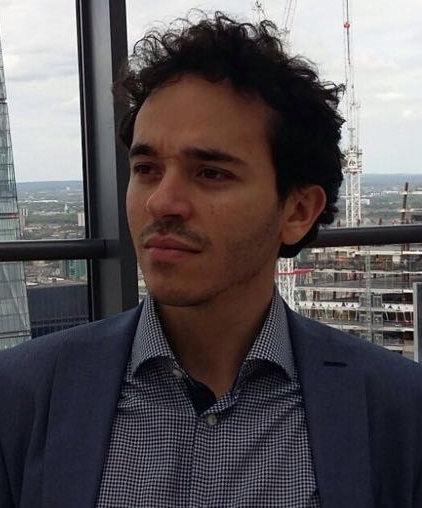
\includegraphics[width=1in,height=1.2in,clip,keepaspectratio]{figs/authors/efalotico.png}}]{Egidio Falotico}
is an Assistant Professor at the BioRobotics Institute at Sant'Anna School of Advanced Studies (SSSA) leading the BRAin Inspired Robotics (BRAIR) Lab. M.Sc. in Computer Science from the University of Pisa, he holds a dual Ph.D. in BioRobotics from the SSSA and in Cognitive Science from the Pierre and Marie Curie University.
\end{IEEEbiography}

%\clearpage
%\pagebreak
\onecolumn
\begin{center}
    \Large
    \textit{Generalized Perturbations} Scenario
\end{center}

All the plot included here are available as interactive html (for proper 3D visualization and zooming) at \url{https://fraiori0.github.io/antip-handover/}, along with videos of the interactions.

\begin{figure*}[h!]
    \centering
    \subfloat[\footnotesize Interaction A.1. The participant takes back the hand after reaching out (as described in Sec. \ref{sec:introduction}), before reaching again for the handover. \label{fig:perturbed:B.2}]{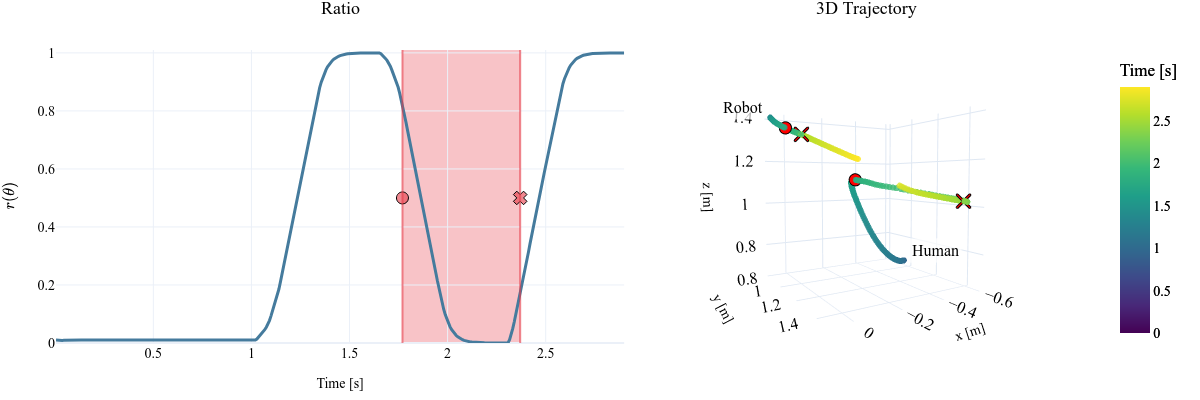
\includegraphics[width=0.65\textwidth]{figs/perturbed_ratio_3d/A.1.png}}
    \\
    \subfloat[\footnotesize Interaction A.2. The participant takes back the hand after reaching out (as described in Sec. \ref{sec:introduction}), before reaching again for the handover. \label{fig:perturbed:B.2}]{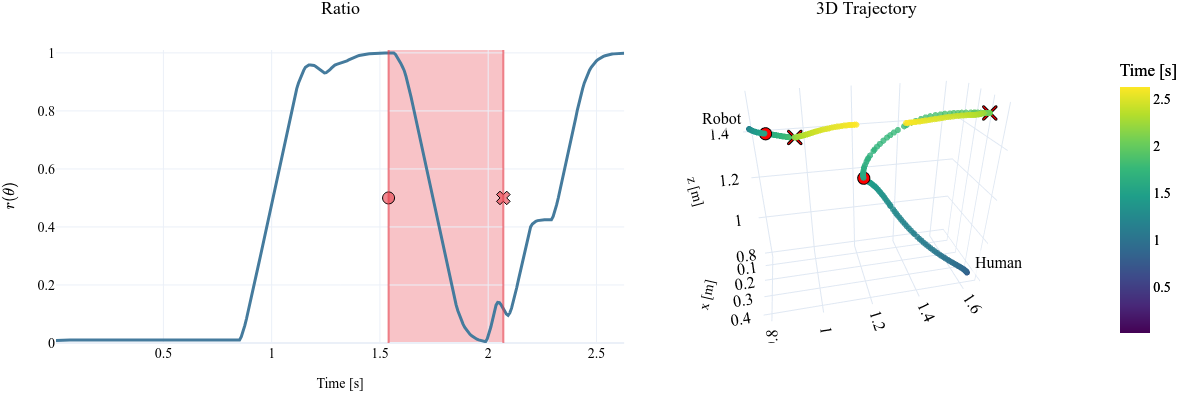
\includegraphics[width=0.65\textwidth]{figs/perturbed_ratio_3d/A.2.png}}
    \\
    \subfloat[\footnotesize Interaction B.1. The participant waves their hand before reaching for the handover. \label{fig:perturbed:B.2}]{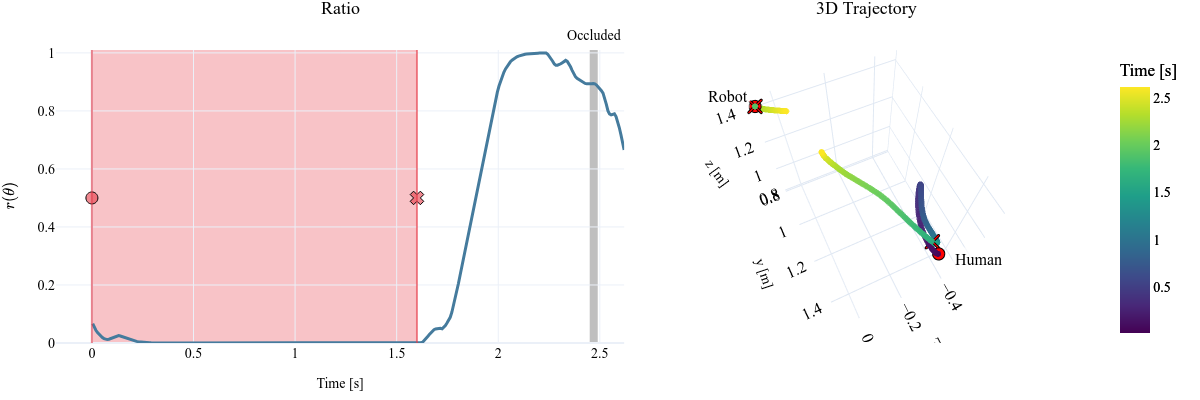
\includegraphics[width=0.65\textwidth]{figs/perturbed_ratio_3d/B.1.png}}
    \\
    \subfloat[\footnotesize Interaction B.2. The participant waves their hand before reaching for the handover. \label{fig:perturbed:B.2}]{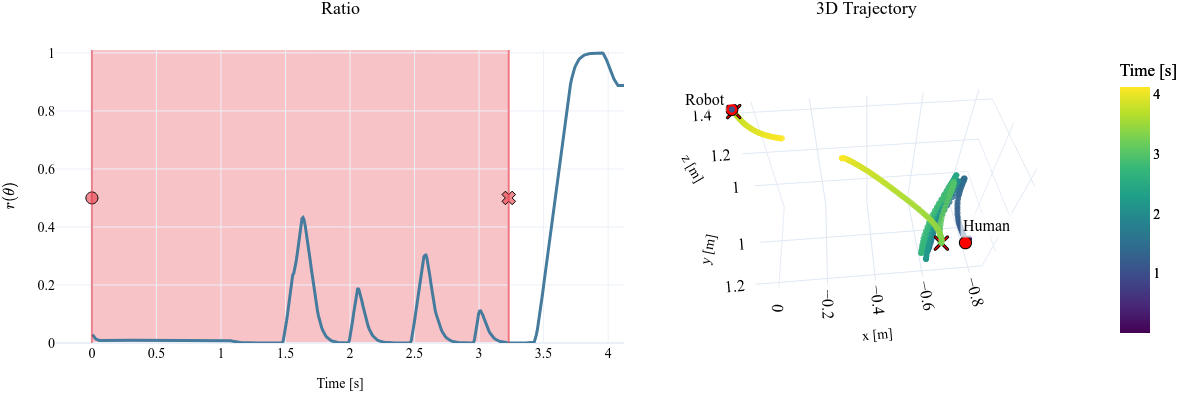
\includegraphics[width=0.65\textwidth]{figs/perturbed_ratio_3d/B.2.png}}
    \hfill
    \caption{Evolution of the ratio and 3D trajectory of interactions A and B in the General Perturbation scenario.
    The red shaded area denotes the time between the start and the end of the perturbation.
    The red circle and cross show the points selected as the start and the end of the perturbation, respectively.
    The color scale denotes corresponding time steps in the two trajectories, with points recorded at the same time as the same color.
    Finally, the gray shaded area denotes part of the interaction where the human hand was occluded; the 3D plot shows a hypothetical interpolated trajectory with small pink markers.
    }
    \label{fig:perturbed:A_B}
\end{figure*}


\begin{figure*}[h!]
    \centering
    \subfloat[\footnotesize Interaction C.1. The participant's hand is slapped. \label{fig:perturbed:2}]{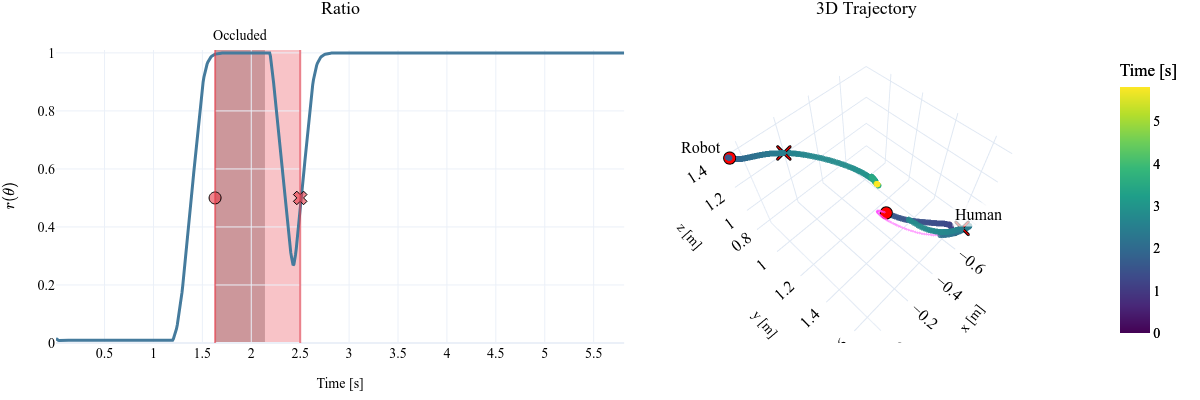
\includegraphics[width=0.65\textwidth]{figs/perturbed_ratio_3d/C.1.png}}
    \\
    \subfloat[\footnotesize Interaction C.2. The participant's hand is slapped. \label{fig:perturbed:2}]{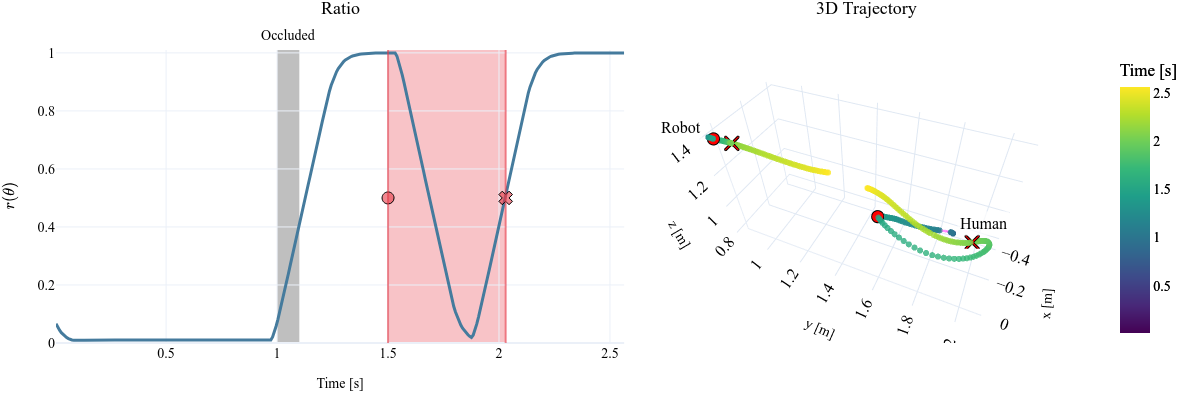
\includegraphics[width=0.65\textwidth]{figs/perturbed_ratio_3d/C.2.png}}
    \\
    \subfloat[\footnotesize Interaction D.1. The participant is thrown a light plastic toy. \label{fig:perturbed:3}]{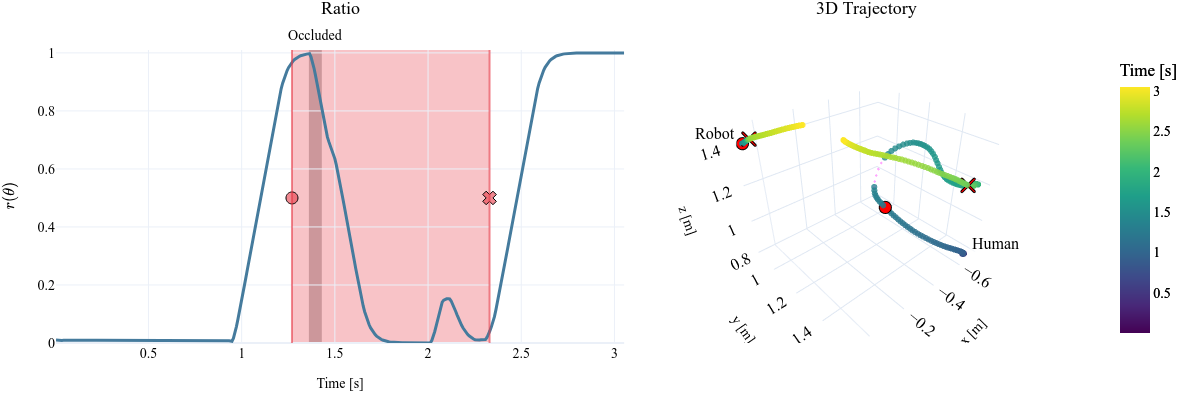
\includegraphics[width=0.65\textwidth]{figs/perturbed_ratio_3d/D.1.png}}
    \\
    \subfloat[\footnotesize Interaction D.2. The participant is thrown a light plastic toy. \label{fig:perturbed:3}]{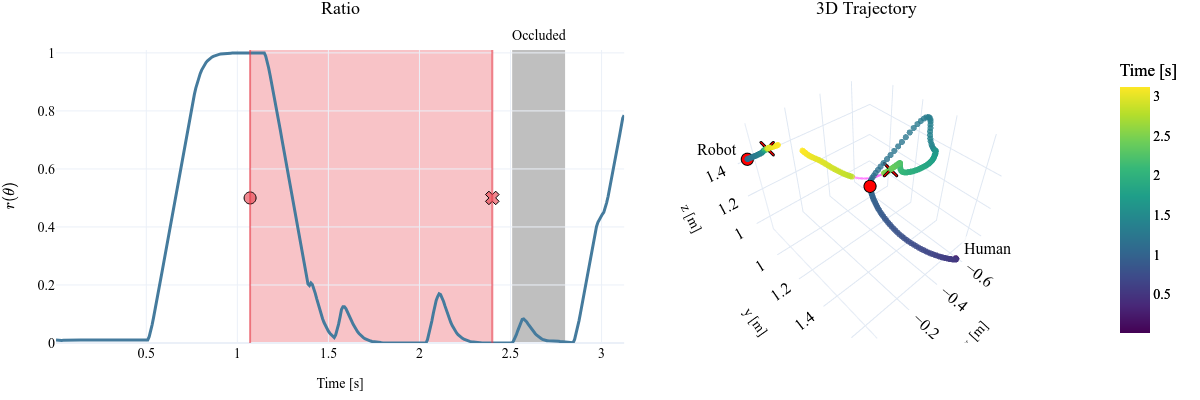
\includegraphics[width=0.65\textwidth]{figs/perturbed_ratio_3d/D.2.png}}
    \hfill
    \caption{Evolution of the ratio and 3D trajectory of interactions C and D in the General Perturbation scenario.
    The red shaded area denotes the time between the start and the end of the perturbation.
    The red circle and cross show the points selected as the start and the end of the perturbation, respectively.
    The color scale denotes corresponding time steps in the two trajectories, with points recorded at the same time as the same color.
    Finally, the gray shaded area denotes part of the interaction where the human hand was occluded; the 3D plot shows a hypothetical interpolated trajectory with small pink markers.
    }
    \label{fig:perturbed:C_D}
\end{figure*}

\begin{figure*}[h!]
    \centering
    \subfloat[\footnotesize Interaction E.1. The participant is thrown a basketball. \label{fig:perturbed:2}]{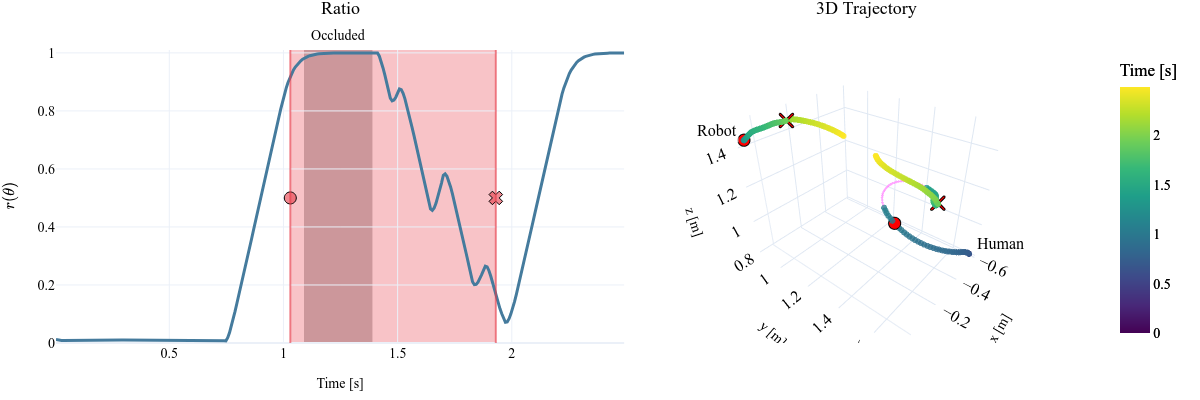
\includegraphics[width=0.65\textwidth]{figs/perturbed_ratio_3d/E.1.png}}
    \\
    \subfloat[\footnotesize Interaction E.2. The participant is thrown a basketball. \label{fig:perturbed:2}]{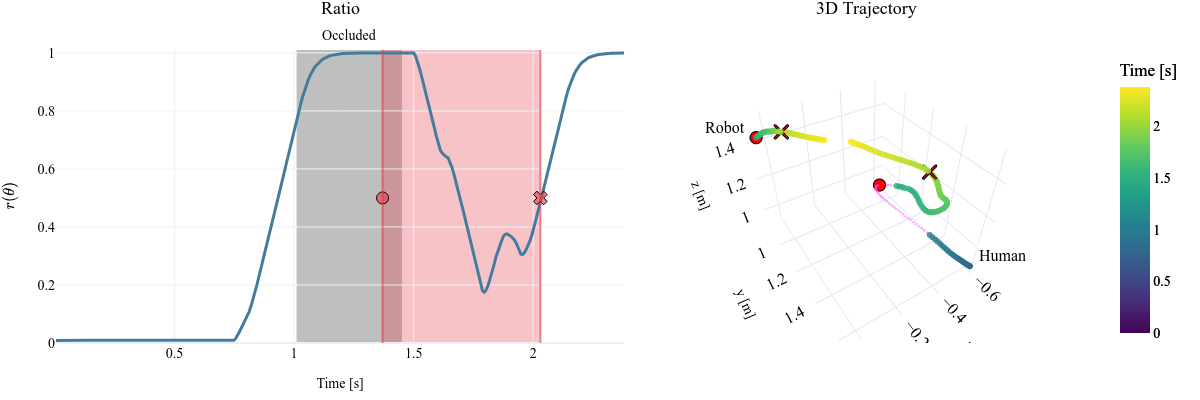
\includegraphics[width=0.65\textwidth]{figs/perturbed_ratio_3d/E.2.png}}
    \\
    \subfloat[\footnotesize Interaction F.1. The participant is thrown a large beanbag. \label{fig:perturbed:3}]{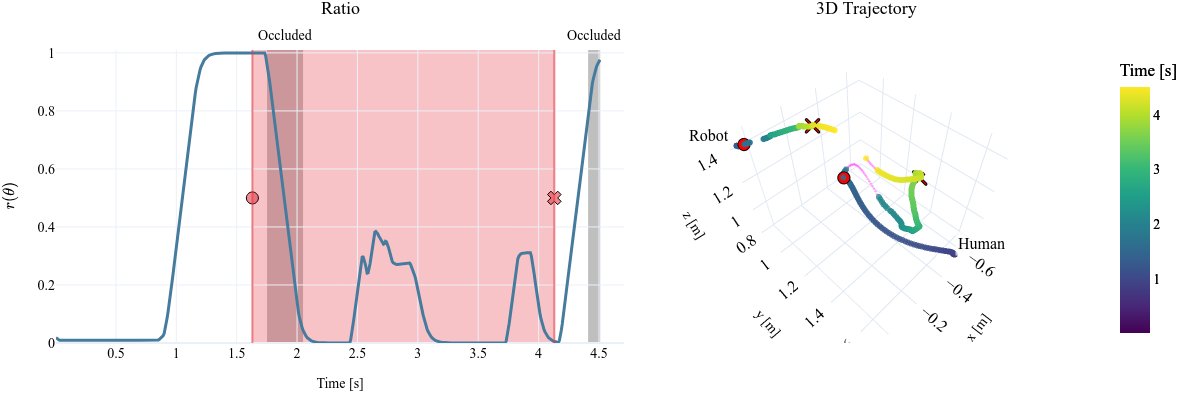
\includegraphics[width=0.65\textwidth]{figs/perturbed_ratio_3d/F.1.png}}
    \\
    \subfloat[\footnotesize Interaction F.2. The participant is thrown a large beanbag. \label{fig:perturbed:3}]{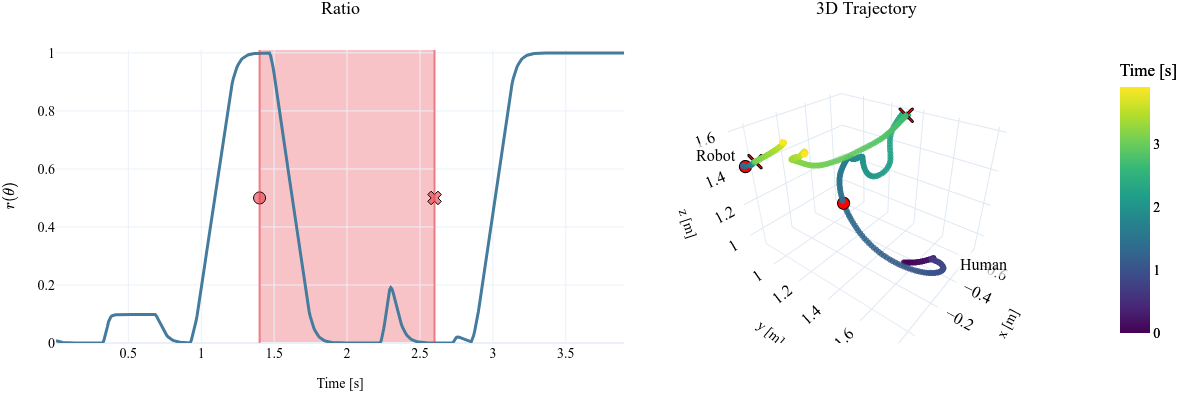
\includegraphics[width=0.65\textwidth]{figs/perturbed_ratio_3d/F.2.png}}
    \hfill
    \caption{Evolution of the ratio and 3D trajectory of interactions E and F in the General Perturbation scenario.
    The red shaded area denotes the time between the start and the end of the perturbation.
    The red circle and cross show the points selected as the start and the end of the perturbation, respectively.
    The color scale denotes corresponding time steps in the two trajectories, with points recorded at the same time as the same color.
    Finally, the gray shaded area denotes part of the interaction where the human hand was occluded; the 3D plot shows a hypothetical interpolated trajectory with small pink markers.
    }
    \label{fig:perturbed:E_F}
\end{figure*}


\end{document}
